
\section{Perintah Navigasi}
Sebelum melakukan perintah navigasi pastikan kita memiliki tools Spyder, anaconda dan selenium. Lakukan instalasi selenium dengan cara ketik "pip install selenium" pada anaconda.

kemudian buka aplikasi Spyder dan masukkan program berikut ini :
\begin{verbatim}
from selenium import webdriver
opsi = webdriver.firefox.options.Options()
opsi.headless = False
binary = webdriver.firefox.firefox_binary.FirefoxBinary(
'C:\\Program Files\\Mozilla Firefox\\firefox.exe')
cap = webdriver.common.desired_capabilities.
DesiredCapabilities().FIREFOX
cap['marionette'] = True
browser=webdriver.Firefox(options=opsi,
capabilities=cap,firefox_binary=binary)
browser.get('https://tokoperhutani.com/')
\end{verbatim}

Penjelasan : 
\begin{enumerate}
	\item From selenium import webdriver Modul selenium webdriver mengimplementasikan kelas yang mendukung berbagai browser termasuk Firefox, Chrome, Internet Explorer, Safari, yang lain, dan RemoteWebDri	ver juga untuk menguji pada browser yang tersedia di mesin jarak jauh. Kita perlu mengimpor webdriver dari paket Selenium untuk menggunakan metode Selenium WebDriver.
	\item Opsi adalah kelas dalam paket webdriver selenium firefox. opts adalah turunan dari kelas Opsi yang dipakai untuk program.
	\item Headless, Python memperbarui instance Options, untuk menyimpan informasi "pengguna ini ingin memulai instance browser headless”.
	\item Webdriver.common.desiredcapabilities.DesiredCapabilities().FIREFOX.   sebagai titik awal untuk membuat objek kemampuan yang diinginkan untuk meminta driver web jarak jauh untuk terhubung ke server selenium.  
	\item Marionette adalah driver otomatisasi untuk mesin Gecko Mozilla.
	\item Browser.get metode akan menavigasi ke halaman yang diberikan oleh URL. WebDriver akan menunggu hingga halaman dimuat penuh (yaitu, "onload" telah diaktifkan) sebelum mengembalikan kontrol ke tes atau skrip.
\end{enumerate}

Setelah anda membuat Tambahan Codingan  seperti diatas untuk merunning program anda tekan run pada bar diatas. Saat kotak yang ditandai pada gambar dibawah, berwarna merah artinya proses running program tersebut masih berjalan. Setelah program di run akan otomatis membuka Mozila Firefox dan akan langsung membuka website tokoperhutani secara otomatis.

\begin{figure}[ht!]
	\centering
	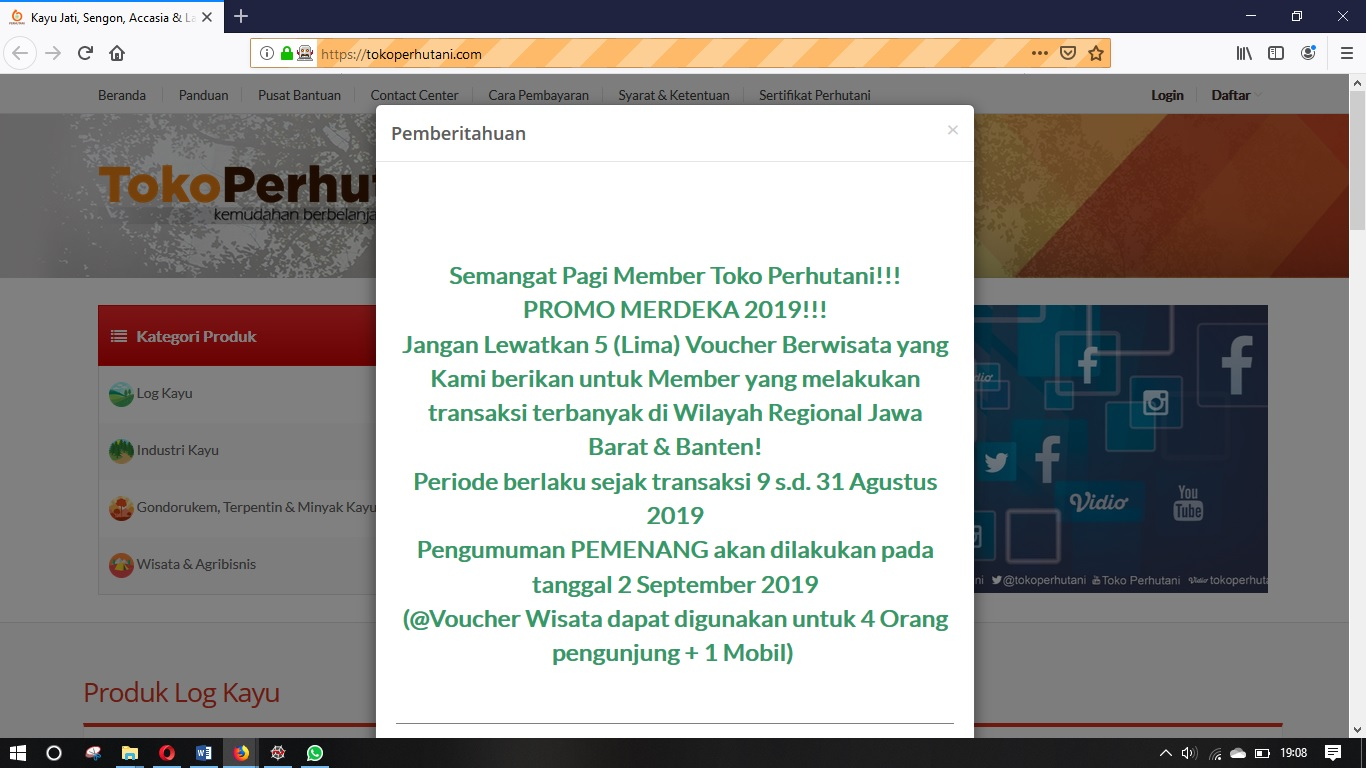
\includegraphics[scale=0.3]{figures/1x}
	\caption{Navigator Pada Menu Beranda}
\end{figure}

Masukkan code berikut untuk test navigator pada menu Cara Pembayaran:

\begin{verbatim}
pembayaran= browser.get('https://tokoperhutani.com/
article/static_art/cara-pembayaran')
\end{verbatim}

Hasilnya  di Mozilla Akan mucul seperti ini :
\begin{figure}[h]
	\centering
	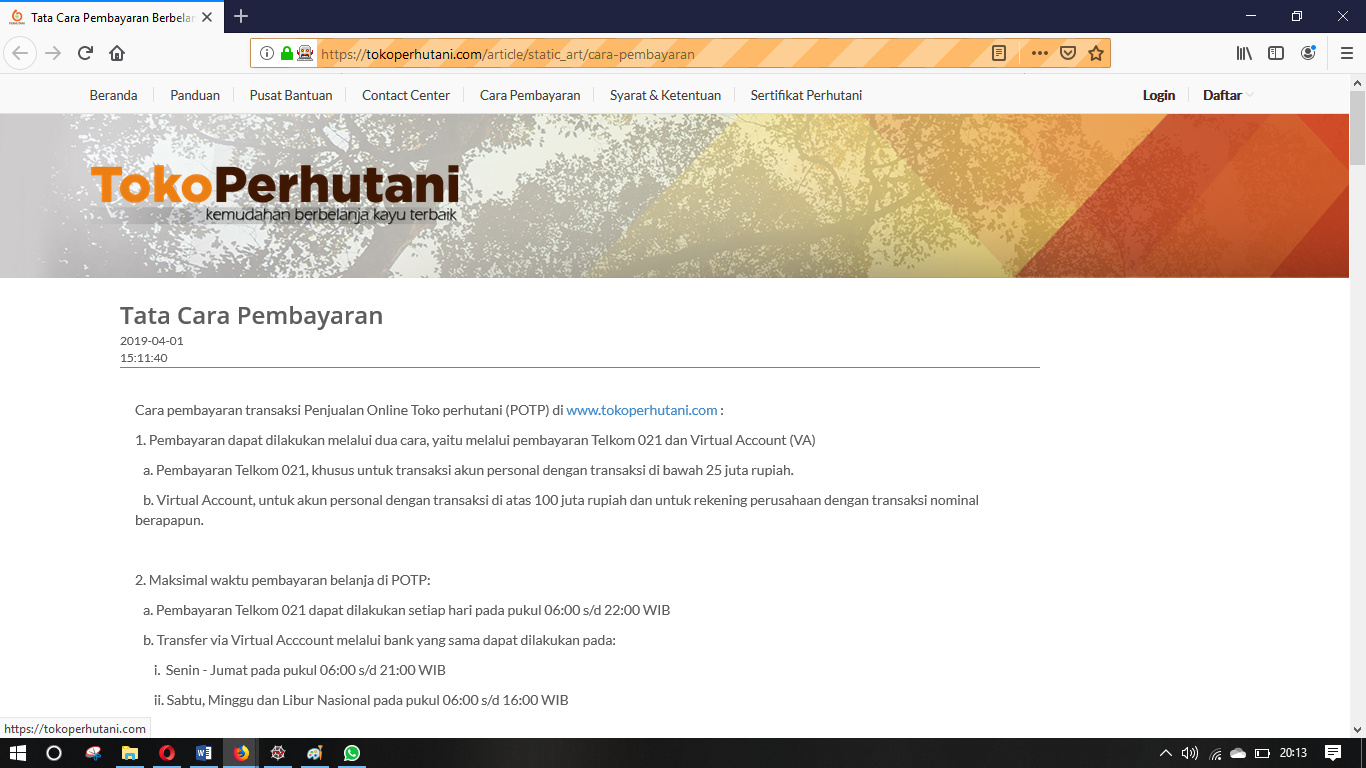
\includegraphics[scale=0.3]{figures/2}
	\caption{Tata Cara Pembayaran}
\end{figure}

Masukkan code berikut untuk test navigator pada menu Sertifikat Perhutani :

\begin{verbatim}
sertperhutani= browser.get('https://tokoperhutani.com/
SertifikatPerhutani')
\end{verbatim}

Hasilnya  di Mozilla Akan mucul seperti ini :
\begin{figure}[h]
	\centering
	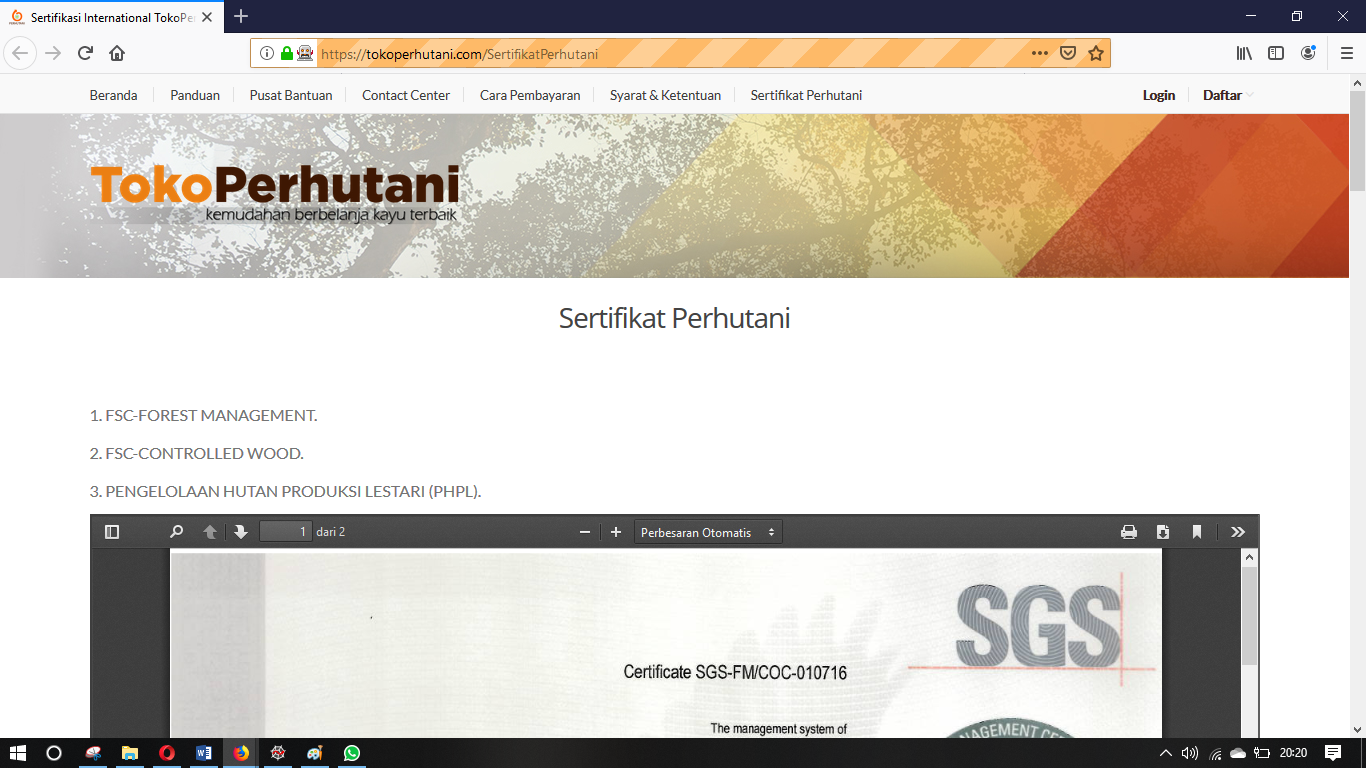
\includegraphics[scale=0.25]{figures/3}
	\caption{Navigator Pada Sertifikat Perhutani}
\end{figure}

Masukkan code berikut untuk test navigator pada menu  Panduan:
\begin{verbatim}
panduan = browser.get('https://tokoperhutani.com/
panduan')
\end{verbatim}

Hasilnya  di Mozilla Akan mucul seperti ini :
\begin{figure}[h]
	\centering
	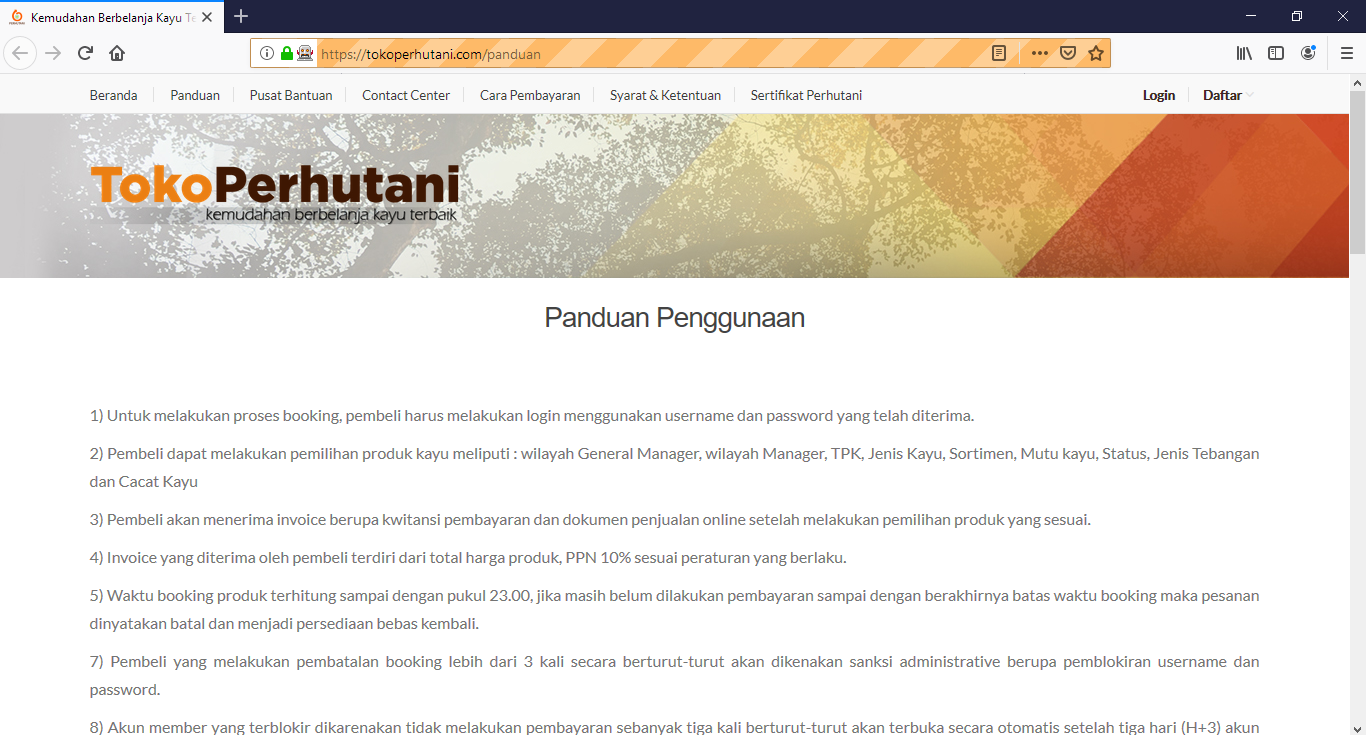
\includegraphics[scale=0.28]{figures/1hasil.PNG}
	\caption{Navigator Pada Panduan}
\end{figure}

Masukkan code berikut untuk test navigator pada menu  Pusat bantuan:
\begin{verbatim}
bantuan = browser.get('https://tokoperhutani.com/
faqs')
\end{verbatim}

Hasilnya  di Mozilla Akan mucul seperti ini :
\begin{figure}[h]
	\centering
	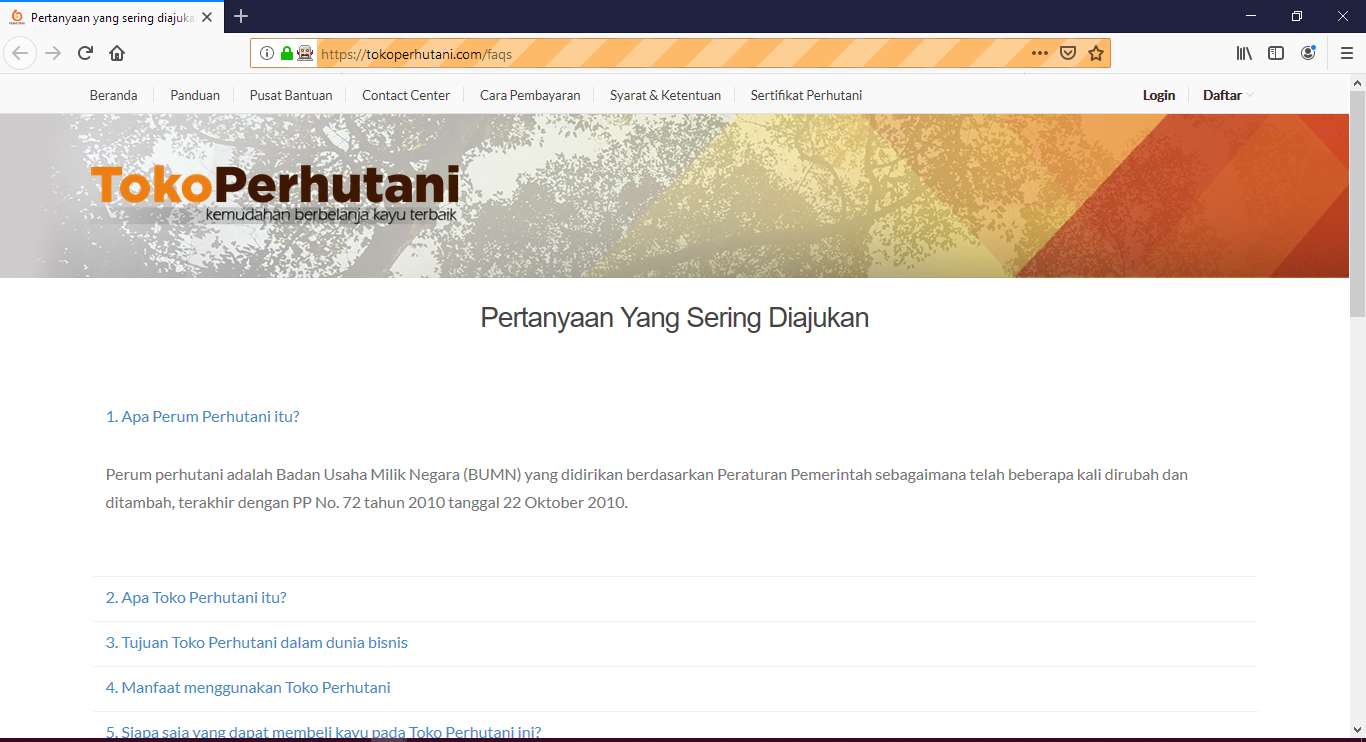
\includegraphics[scale=0.3]{figures/2hasil.PNG}
	\caption{Navigator Pada Pusat Bantuan}
\end{figure}

Masukkan code berikut untuk test navigator pada menu  Alamat kantor:
\begin{verbatim}
alamat = browser.get('https://tokoperhutani.com/
article/detil/alamat-kantor')
\end{verbatim}

Hasilnya  di Mozilla Akan mucul seperti ini :
\begin{figure}[h]
	\centering
	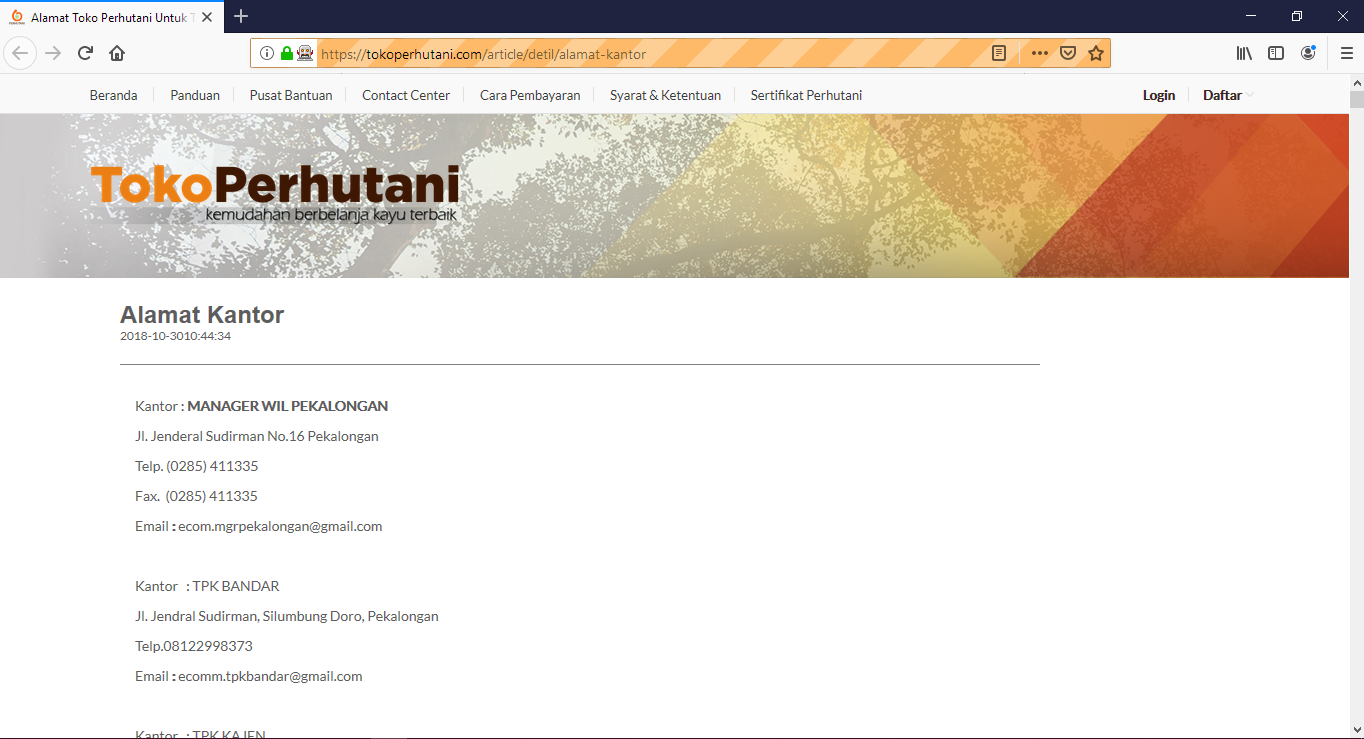
\includegraphics[scale=0.3]{figures/3hasil.PNG}
	\caption{Navigator Pada Alamat Kantor}
\end{figure}


Masukkan code berikut untuk test navigator ke halaman panduan Registrasi:
\lstinputlisting[language=Python, firstline=3, lastline=3, caption=Halaman Panduan Registrasi]{src/dinda.py}

Hasilnya  di Google Chrome Akan mucul seperti ini :
\begin{figure}[h]
	\centering
	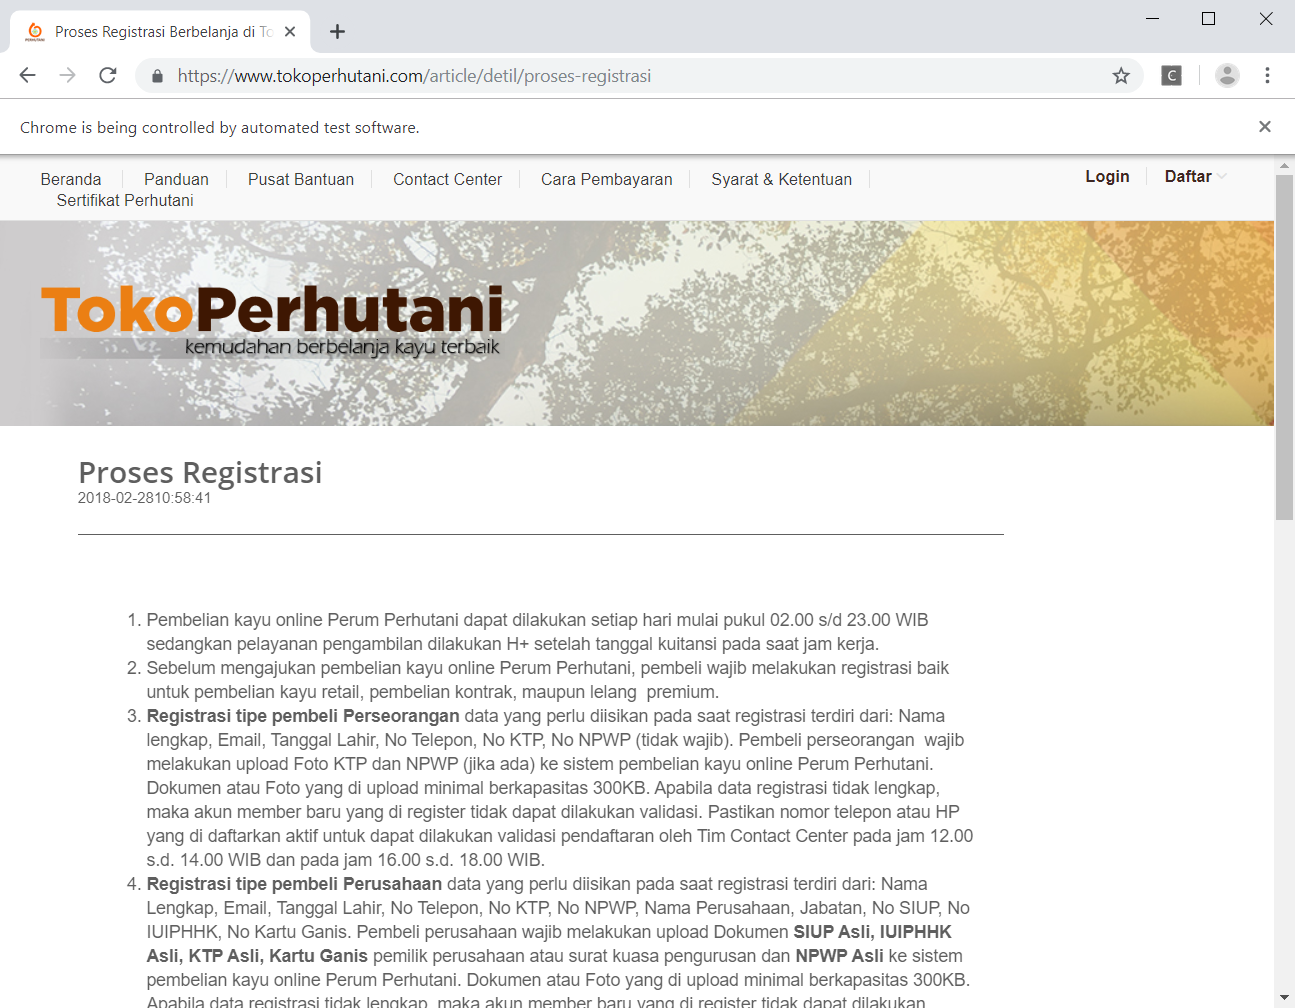
\includegraphics[scale=0.23]{figures/1pdregis}
	\caption{Halaman Panduan Registrasi}
\end{figure}

Masukkan code berikut untuk test menampilkan pilihan pendaftaran:
\lstinputlisting[language=Python, firstline=5, lastline=5, caption=Tombol Navigasi Daftar]{src/dinda.py}

Hasilnya  di Google Chrome Akan mucul seperti ini :
\begin{figure}[h]
	\centering
	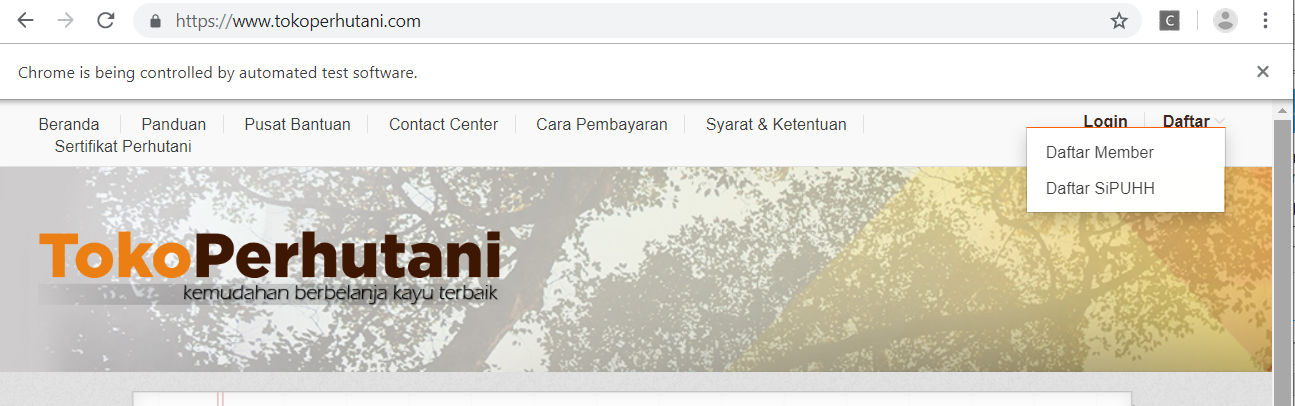
\includegraphics[scale=0.42]{figures/2daftar}
	\caption{Tombol Navigasi Daftar}
\end{figure}

Masukkan code berikut untuk test memilih Daftar Member:
\lstinputlisting[language=Python, firstline=7, lastline=7, caption=Halaman Daftar Member]{src/dinda.py}

Hasilnya  di Google Chrome Akan mucul seperti ini :
\begin{figure}[h]
	\centering
	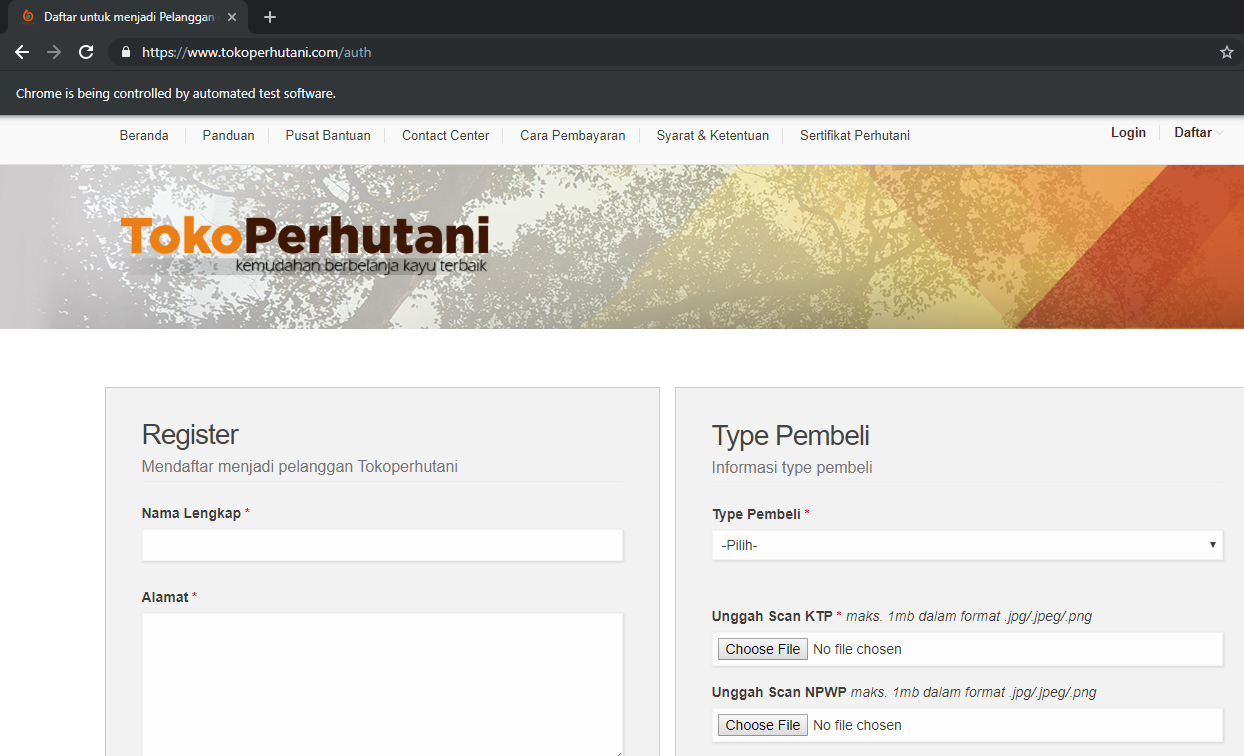
\includegraphics[scale=0.33]{figures/3daftar}
	\caption{Halaman Daftar Member}
\end{figure}

Masukkan code berikut untuk test navigator ke halaman Contact Center:
\lstinputlisting[language=Python, firstline=9, lastline=9, caption=Halaman Contact Center]{src/dinda.py}

Hasilnya  di Google Chrome Akan mucul seperti ini :
\begin{figure}[h]
	\centering
	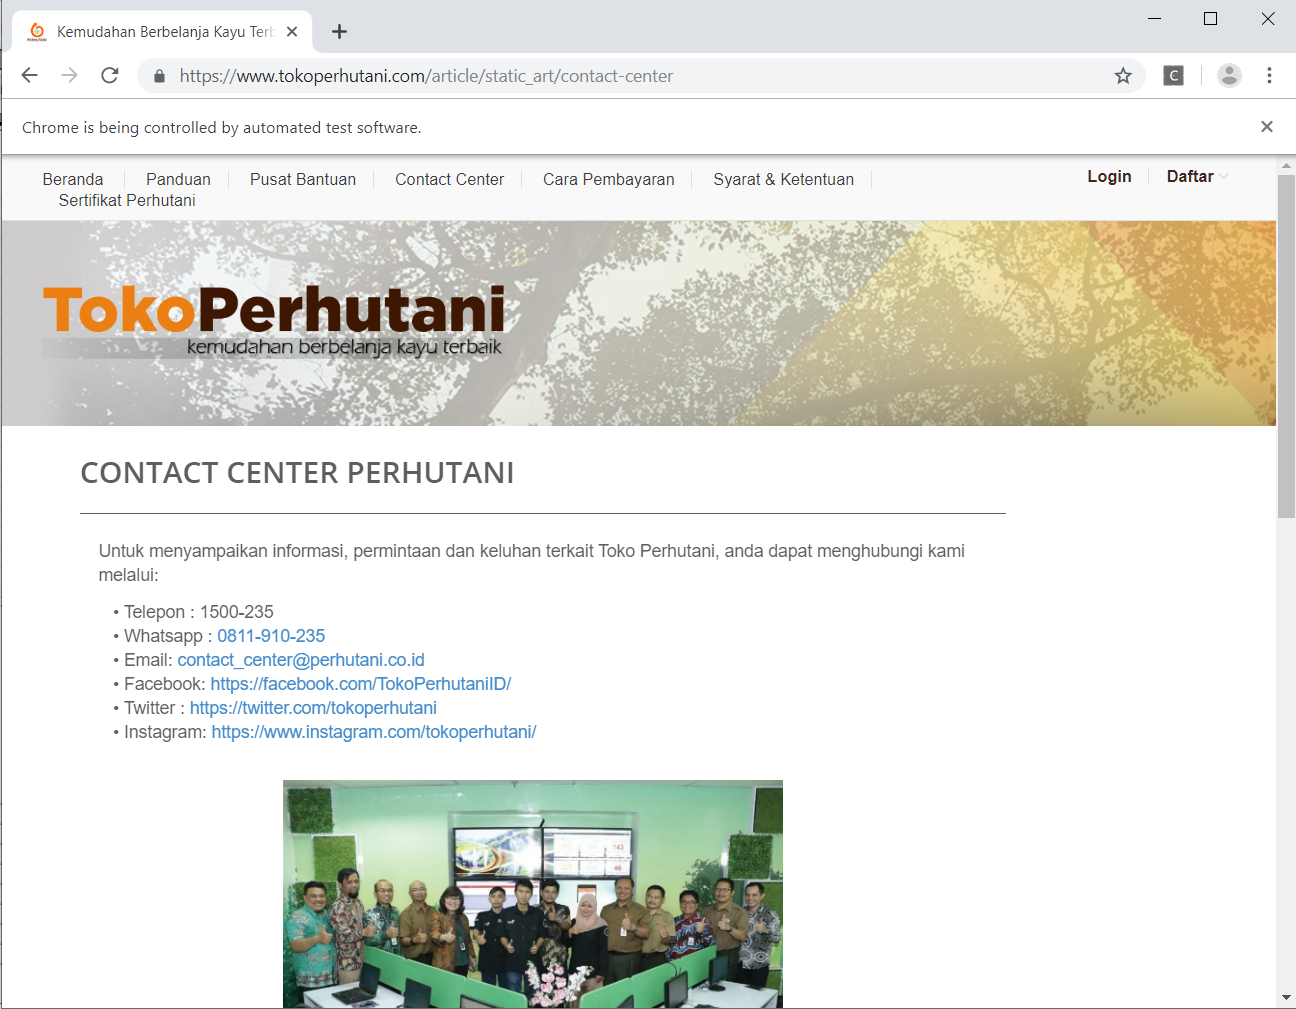
\includegraphics[scale=0.3]{figures/4kontak}
	\caption{Halaman Contact Center}
\end{figure}

Masukkan code berikut untuk test navigator pada menu Kayu Pinus:

\begin{verbatim}
KayuPinus = browser.get('https://tokoperhutani.com/
article/detil/kayu-pinus'
\end{verbatim}

Hasilnya  di Mozilla Akan mucul seperti ini :
\begin{figure}[h]
	\centering
	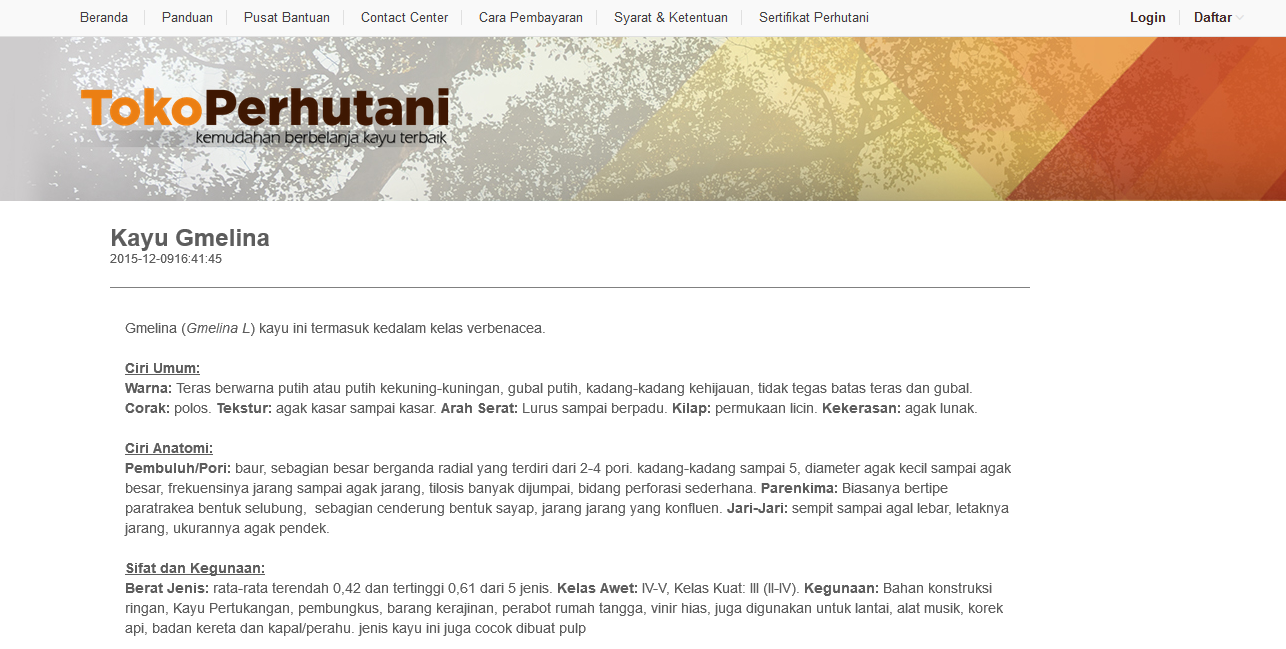
\includegraphics[scale=0.29]{figures/aa}
	\caption{Kayu Pinus}
\end{figure}

Masukkan code berikut untuk test navigator pada menu Kayu Gamelina :
\begin{verbatim}
KayuGmelina = browser.get('https://tokoperhutani
.com/article/detil/kayu-gmelina'
\end{verbatim}

Hasilnya  di Mozilla Akan mucul seperti ini :
\begin{figure}[h]
	\centering
	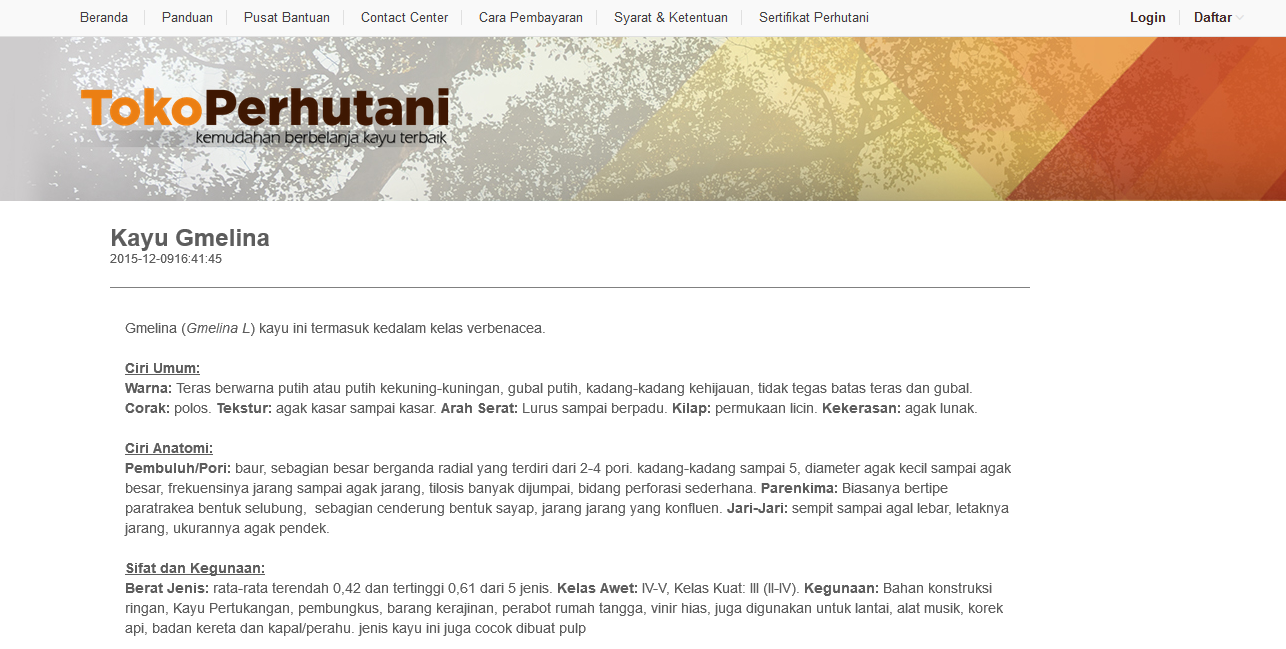
\includegraphics[scale=0.342]{figures/2kg}
	\caption{Kayu Gamelina}
\end{figure}

Masukkan code berikut untuk test navigator pada menu Kayu Sonokeling :
\begin{verbatim}
KayuSonokeling = browser.get('https://tokoperhu
tani.com/article/detil/kayu-sonokeling'
\end{verbatim}

Hasilnya  di Mozilla Akan mucul seperti ini :
\begin{figure}[h]
	\centering
	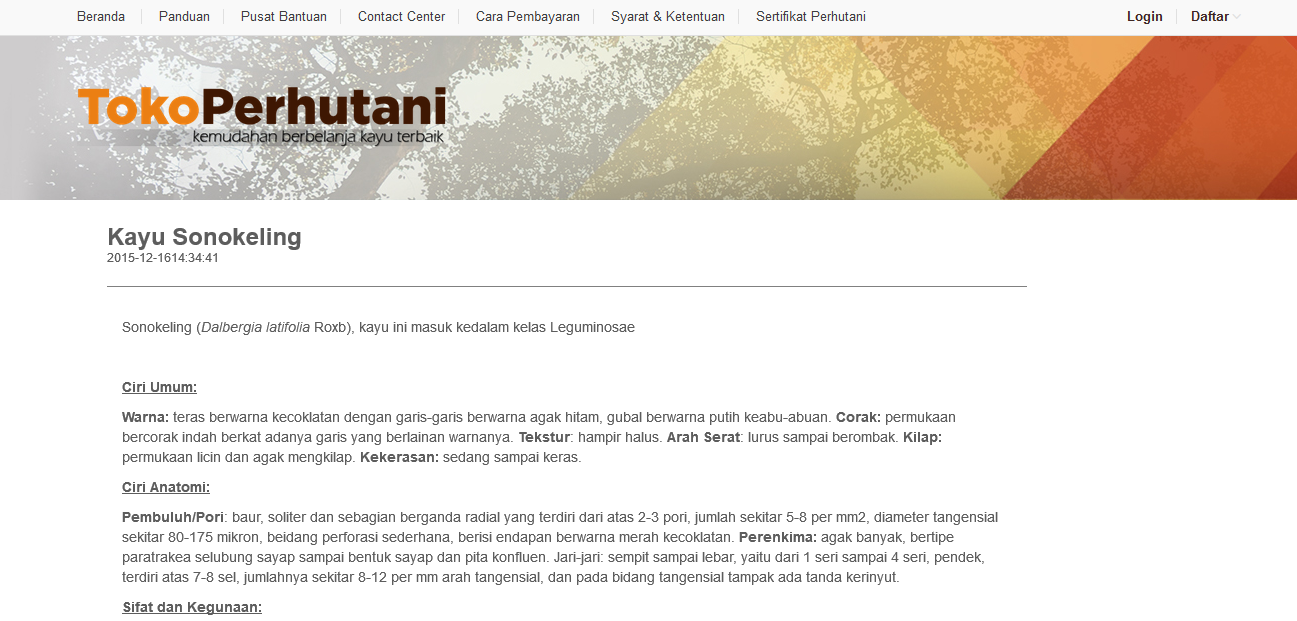
\includegraphics[scale=0.332]{figures/cc}
	\caption{Kayu Sonokeling}
\end{figure}

Masukkan code berikut untuk test navigator pada menu Kayu Pinus :
\begin{verbatim}
kayupinus = browser.get('https://www.tokoperhu
tani.com/article/detil/kayu-pinus')
\end{verbatim}

Hasilnya  di Mozilla Akan mucul seperti ini :
\begin{figure}[h]
	\centering
	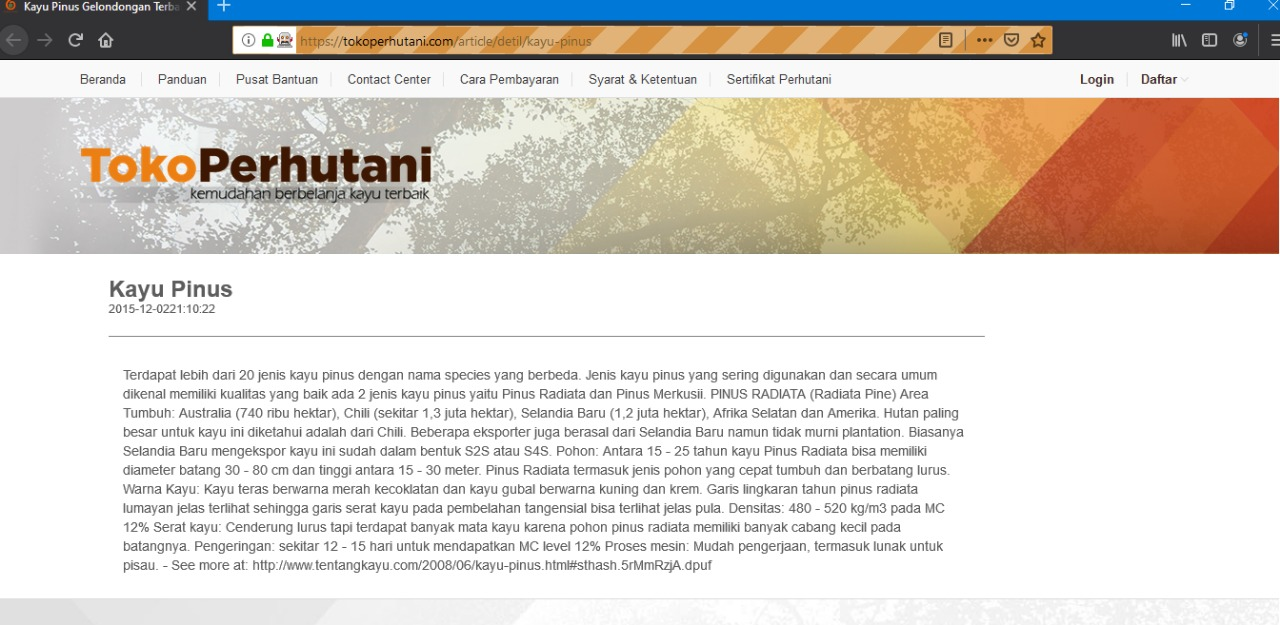
\includegraphics[scale=0.25]{figures/j1}
	\caption{Kayu Pinus}
\end{figure}

Masukkan code berikut untuk test navigator pada menu Kayu Gmelina :
\begin{verbatim}
kayugmelina  = browser.get('https://www.toko
perhutani.com/article/detil/kayu-gmelina')
\end{verbatim}

Hasilnya  di Mozilla Akan mucul seperti ini :
\begin{figure}[h]
	\centering
	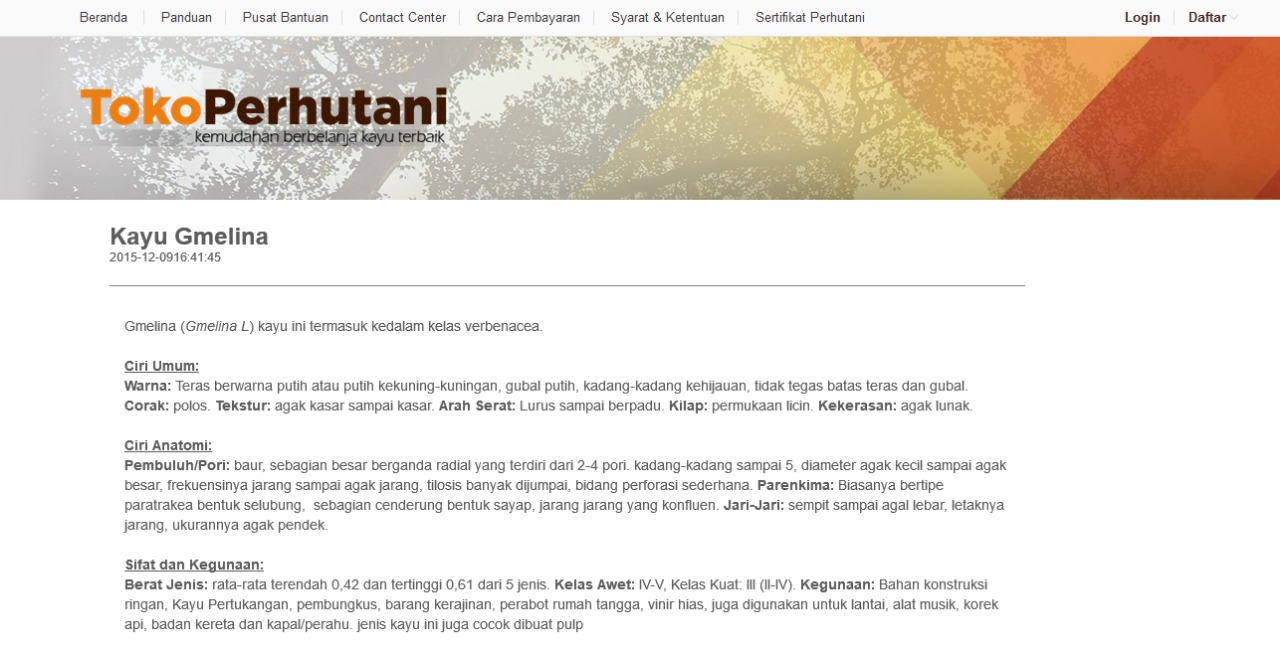
\includegraphics[scale=0.255]{figures/j2}
	\caption{Kayu Gmelina}
\end{figure}

Masukkan code berikut untuk test navigator pada menu Kayu Sonokeling :
\begin{verbatim}
kayusonokeling =  browser.get('www.tokoper
hutani.com/article/detil/kayu-sonokeling')
\end{verbatim}

Hasilnya  di Mozilla Akan mucul seperti ini :
\begin{figure}[h]
	\centering
	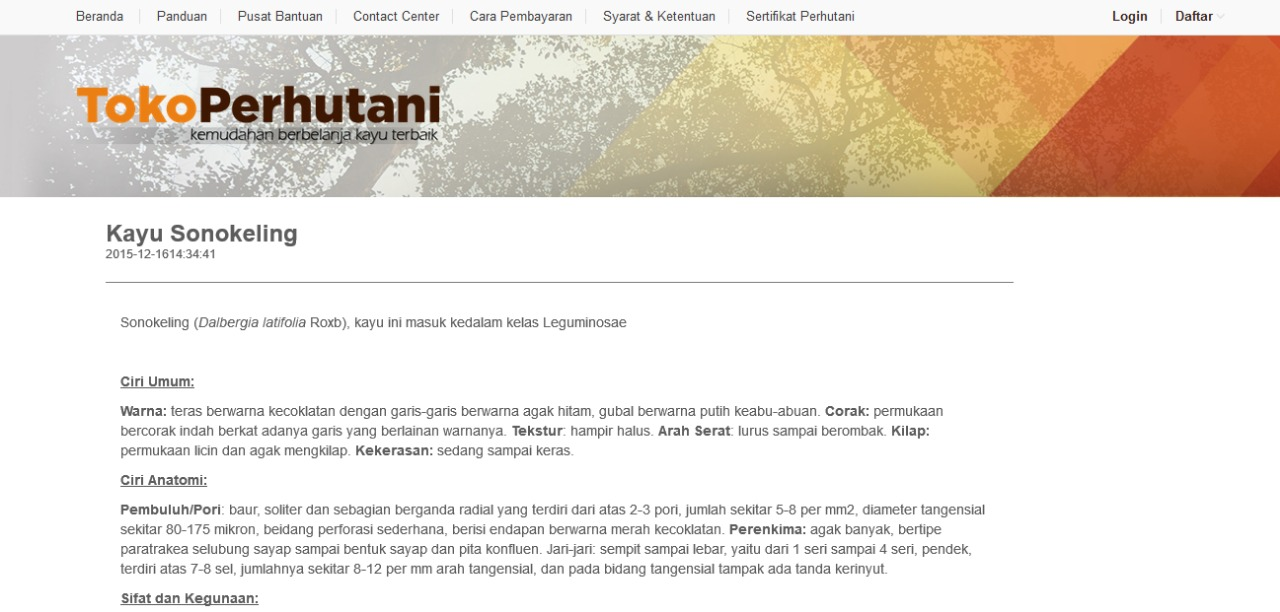
\includegraphics[scale=0.25]{figures/j3}
	\caption{Kayu Sonokeling}
\end{figure}

\newpage
\section{Pendaftaran Member}
Pada tutorial ini membutuhkan file gambar ktp untuk verifikasi data.

Masukan kode dibawah ini yang berfungsi untuk meng-import modul selenium dan time.

\lstinputlisting[language=Python, firstline=13, lastline=21, caption=Import Modul]{src/dinda.py}

Penjelasan:
\begin{enumerate}
	\item mengimport modul selenium dan time.
	\item lalu tahap selanjutnya membuka webdriver chrome / firefox dan membuka link web perhutani.
	\item karena di halaman landing page web toko perhutani terdapat modal yang menutupi halaman disini kita menutupnya.
\end{enumerate}

\pagebreak
Hasilnya tampilan beranda awal website tokoperhutani:


\begin{figure}[h]
	\centering
	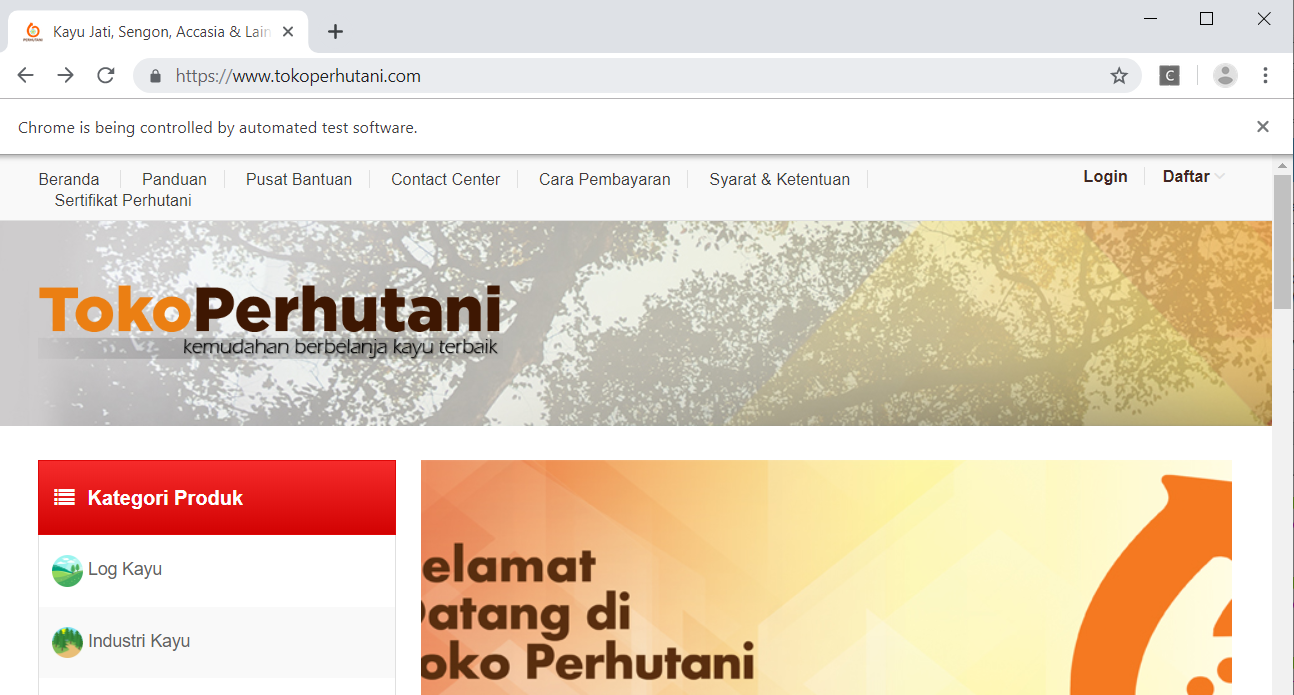
\includegraphics[scale=0.425]{figures/1home}
	\caption{Navigator Pada Menu Beranda}
\end{figure}

Masukkan code berikut untuk test masuk menu pendaftaran dengan menekan tombol daftar lalu memilih daftar member :
\lstinputlisting[language=Python, firstline=23, lastline=25, caption=Halaman Daftar]{src/dinda.py}

Hasilnya  di Google Chrome akan mucul seperti ini :
\begin{figure}[h]
	\centering
	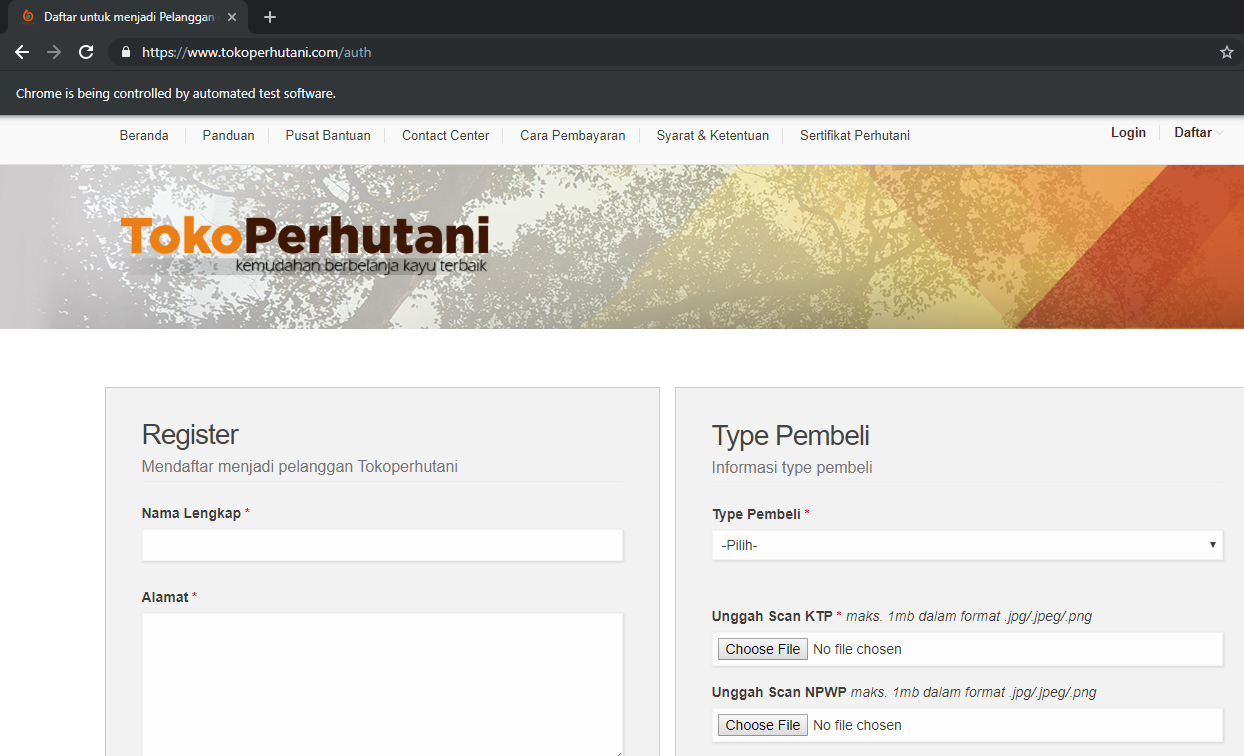
\includegraphics[scale=0.25]{figures/3daftar}
	\caption{Halaman Daftar}
\end{figure}

\pagebreak
Masukkan code berikut untuk test mengisi form nama, alamat dan lain-lain :
\lstinputlisting[language=Python, firstline=27, lastline=36, caption=Mengisi Form]{src/dinda.py}


Hasilnya akhir pada Google Chrome Akan mucul seperti ini:
\begin{figure}[h]
	\centering
	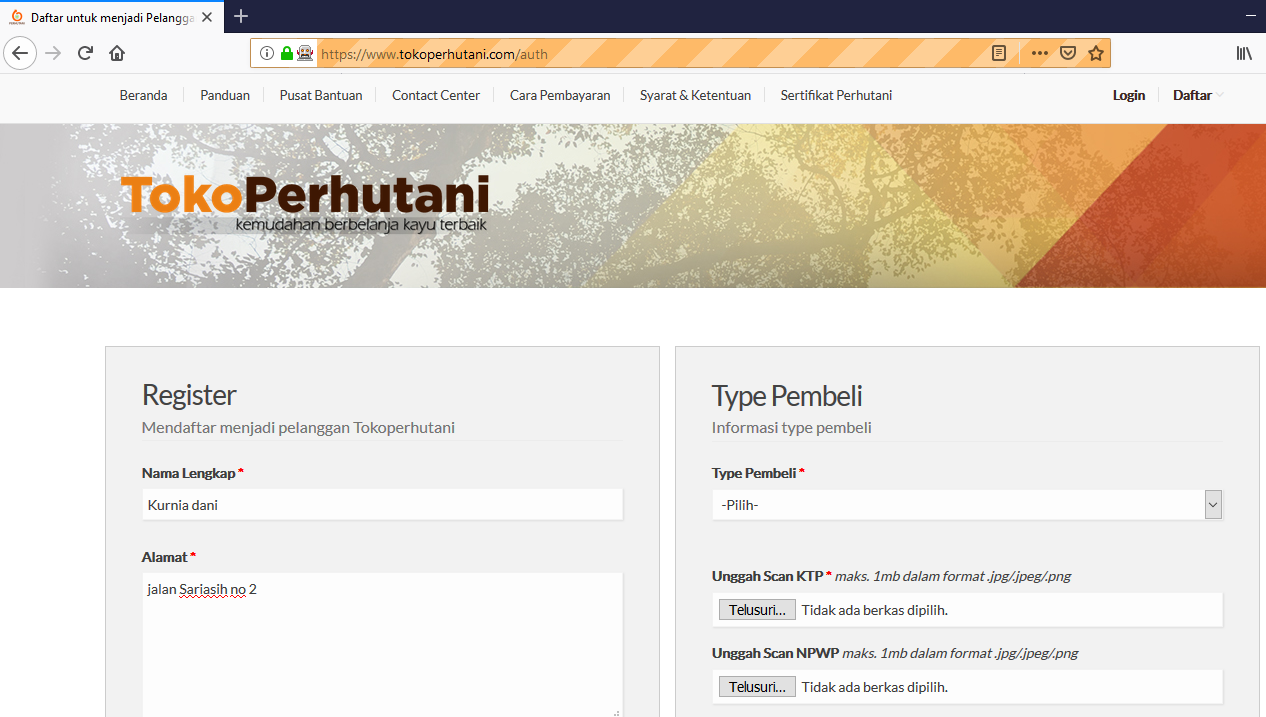
\includegraphics[scale=0.30]{figures/4daftar}
	\caption{Halaman Mengisi Form}
\end{figure}

Apabila telah selesai melakukan pendaftaran, selanjutnya akan ada verifikasi dari pihak Tokoperhutani sehari setelah pendaftaran dilakukan.

\newpage
\section{Reset Password, Login Dan Menghubungi Contact Person di WA WA}
\subsection{Login}
Selanjutnya kita akan mencoba untuk melakukan login pada tool dengan selenium. 
Masukkan kode berikut untuk menampilkan form login:
\begin{verbatim}
content..browser.find_element_by_xpath('/html/body/div/
nav/div/div[2]/ul/li[1]/a/strong').click().
\end{verbatim}



Berikut hasil dari codingan di atas:
\begin{figure}[h]
	\centering
	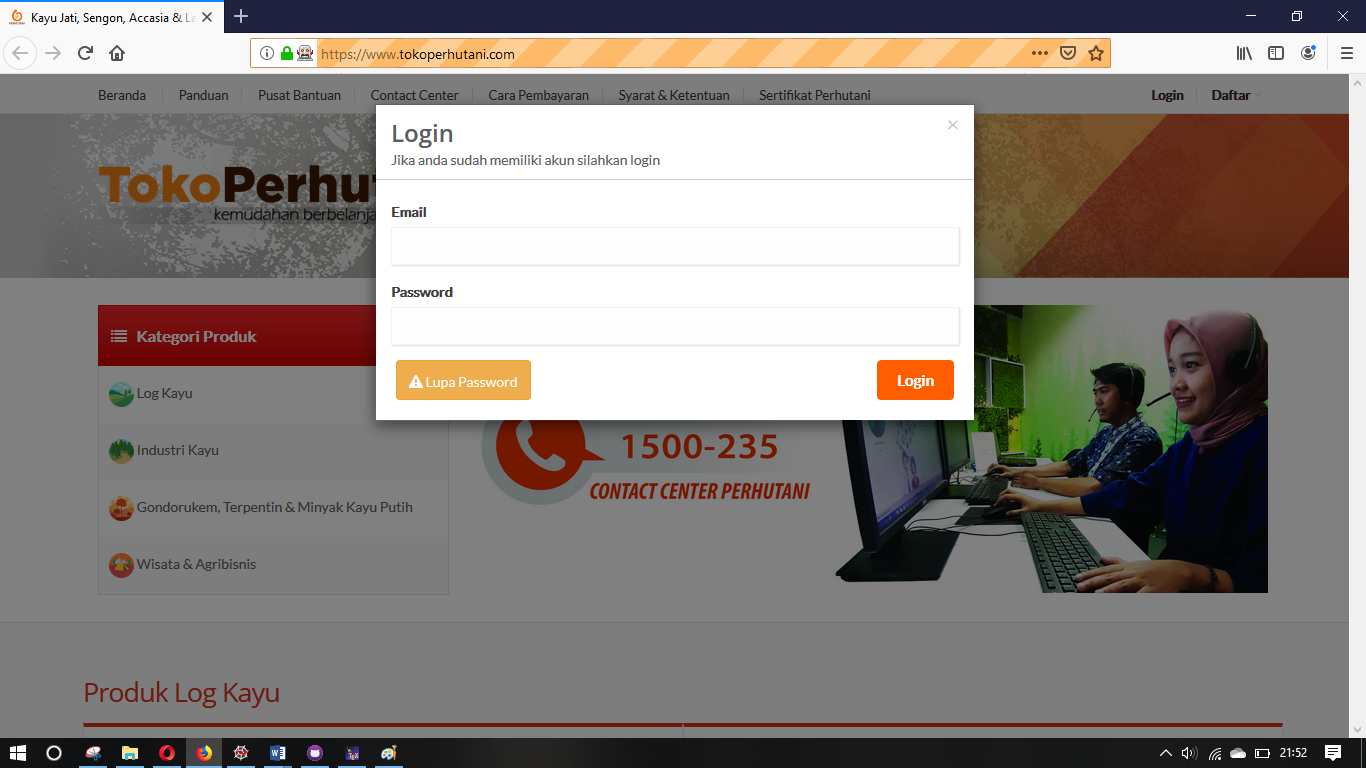
\includegraphics[scale=0.20]{figures/0login}
	\caption{Halaman Login}
\end{figure}

kemudian tambahkan kode berikut untuk memasukkan email, password dan tombol untuk mengclick login secara otomatis: 
\begin{verbatim}
browser.find_element_by_id('email').
send_keys('nsfthrn@gmail.com')

browser.find_element_by_id('password').
send_keys("C4CA2F")

browser.find_element_by_class_name('le-button').click() 
\end{verbatim}
\newpage
Kemudian akan muncul proses login seperti berikut:
\begin{figure}[h]
	\centering
	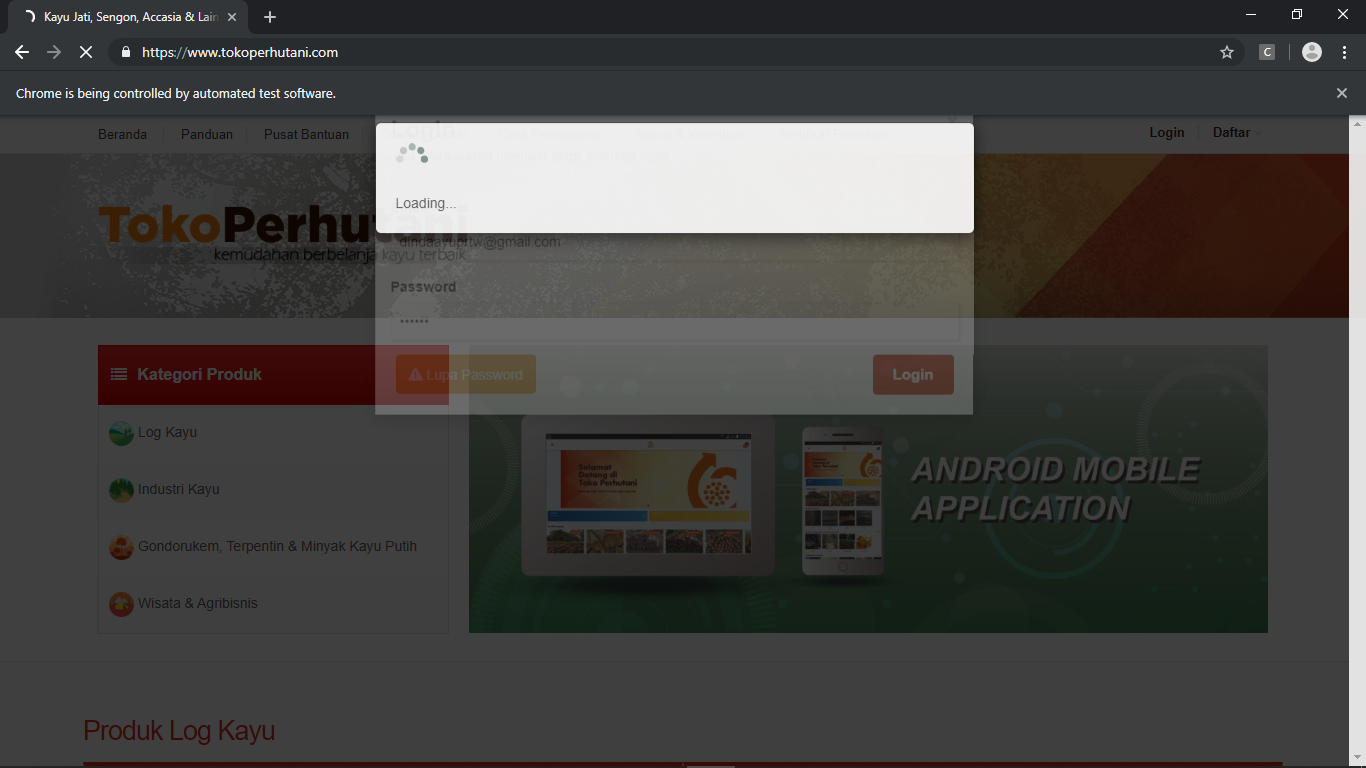
\includegraphics[scale=0.21]{figures/1login}
	\caption{Proses Login}
\end{figure}

Setelah proses loading selesai maka Login berhasil dan akan muncul tampilan seperti berikut:
\begin{figure}[h]
 	\centering
 	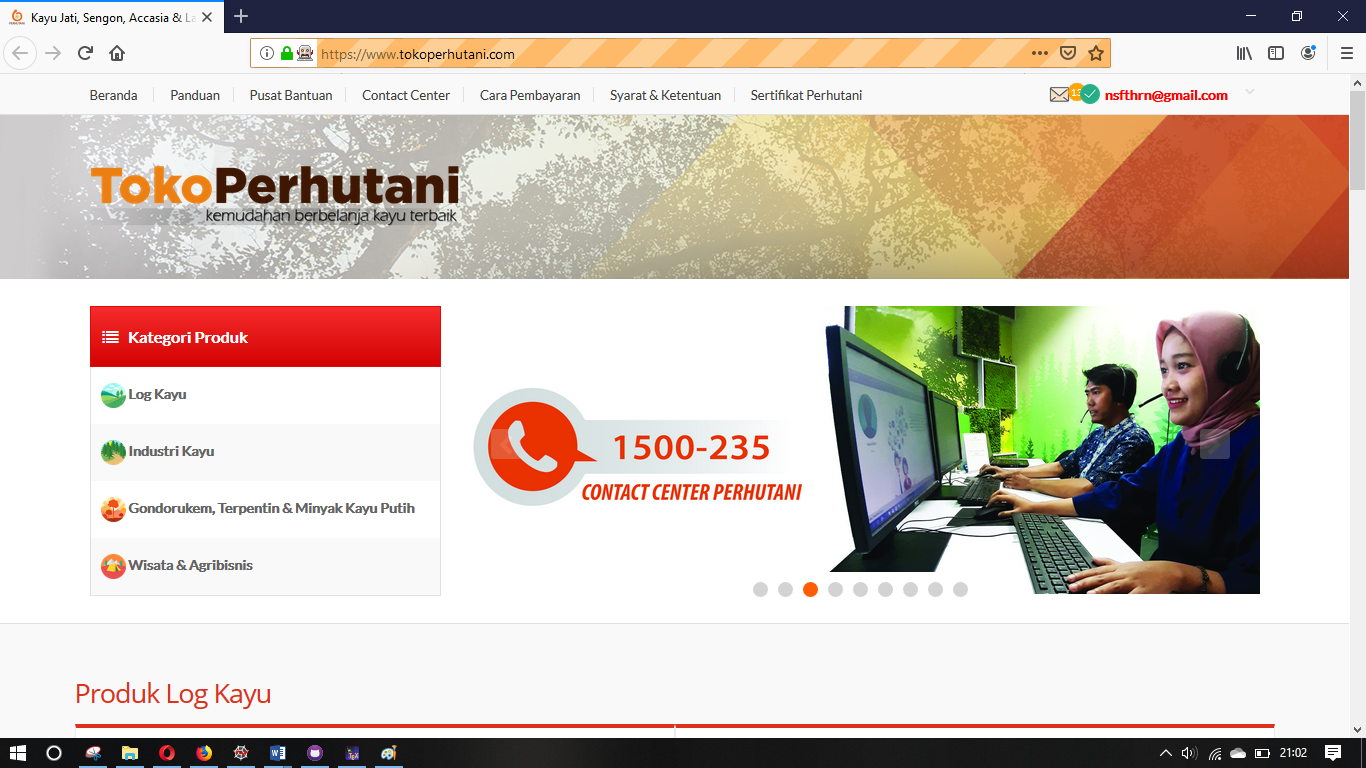
\includegraphics[scale=0.20]{figures/2login}
 	\caption{Login Berhasil}
\end{figure}

\newpage
\subsection{Reset Password}
Setelah kita login langkah selanjutnya adalah reset password, sebelumnya kita tekan tombol ganti password berikut terlebih dahulu,masukkan code berikut:

\begin{verbatim}
browser.find_element_by_xpath('/html/body/div/nav/div/div[2]
/ul/strong/li/a/strong').click()
\end{verbatim} 

Hasil setelah kita klik tombol Ganti Password adalah sebagai berikut: 
\begin{figure}[h]
	\centering
	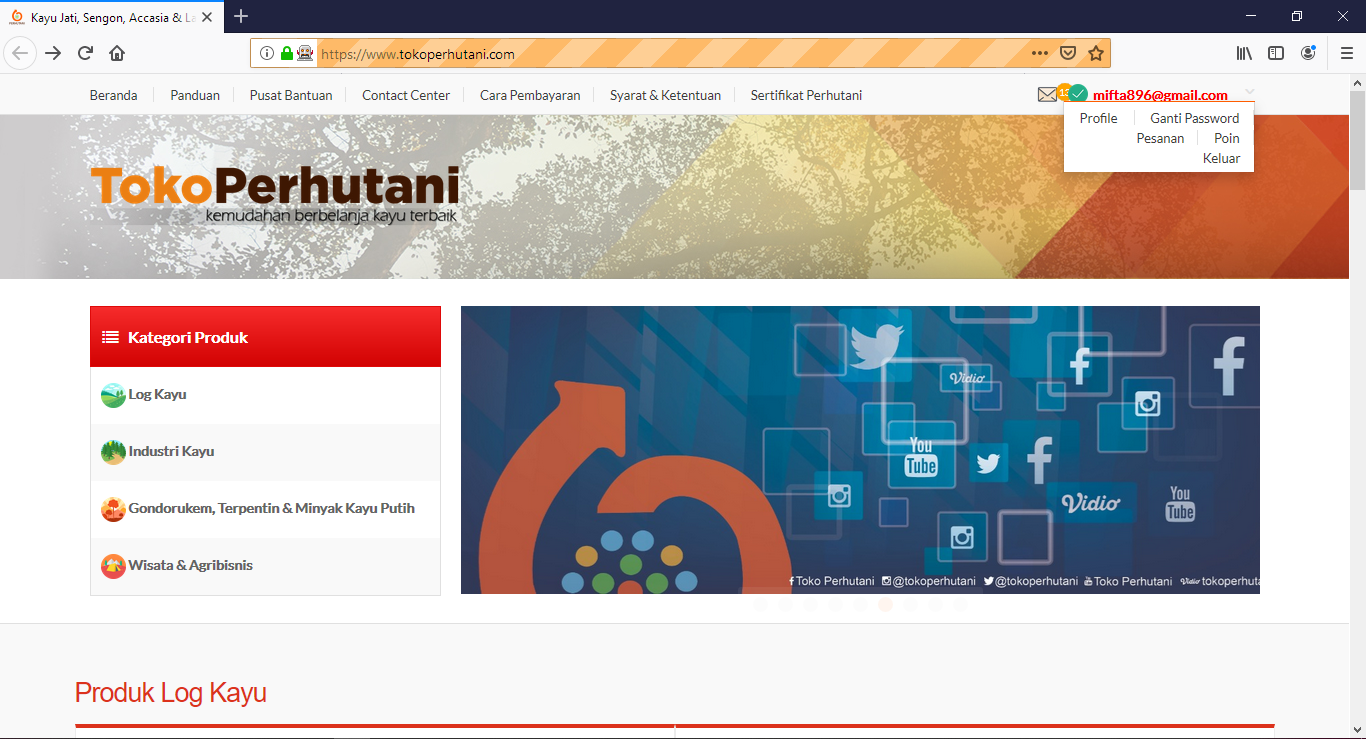
\includegraphics[scale=0.32]{figures/1GantiPassword}
	\caption{Halaman Utama}
\end{figure}


Setelah kita mengklik tombol ganti password langkah selanjutnya adalah kita mengganti password, langkah nya adalah sebagai berikut, masukkan kodingan berikut: 
\begin{verbatim}
browser.find_element_by_xpath('/html/body/div/
nav/div/div[2]/ul/strong/li/ul/li[2]/a').clicl()
\end{verbatim} 

\newpage
Hasil setelah kita klik ganti password adalah sebagai berikut: 
\begin{figure}[h]
	\centering
	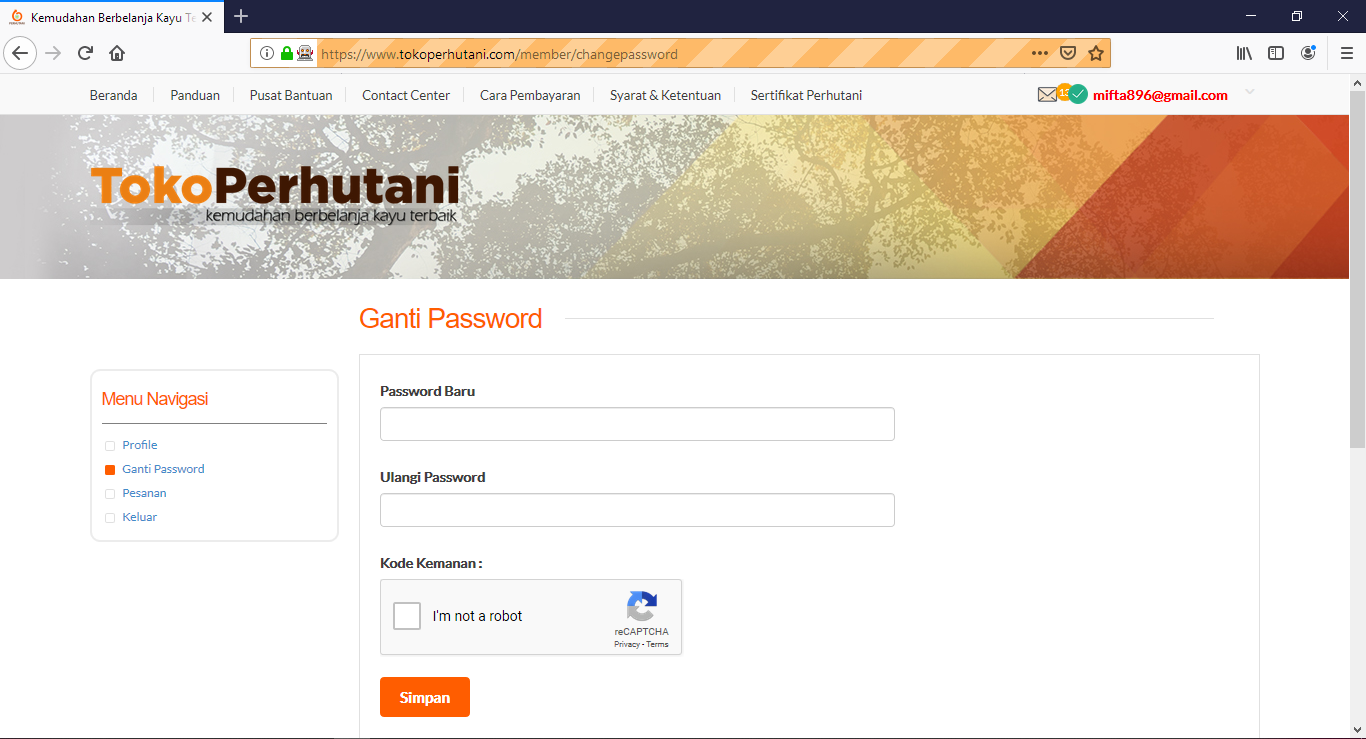
\includegraphics[scale=0.25]{figures/2GantiPassword}
	\caption{Halaman Reset Password}
\end{figure}

langkah selanjutnya adalah kita ganti password, masukkan kodingan berikut: 
\begin{verbatim}
browser.find_element_by_name('user_pass1').send_keys
('mifta@22')
browser.find_element_by_name('user_pass2').send_keys
('mifta@22')
\end{verbatim}

Hasil setelah kita mengganti password adalah sebagai berikut: 
\begin{figure}[h]
	\centering
	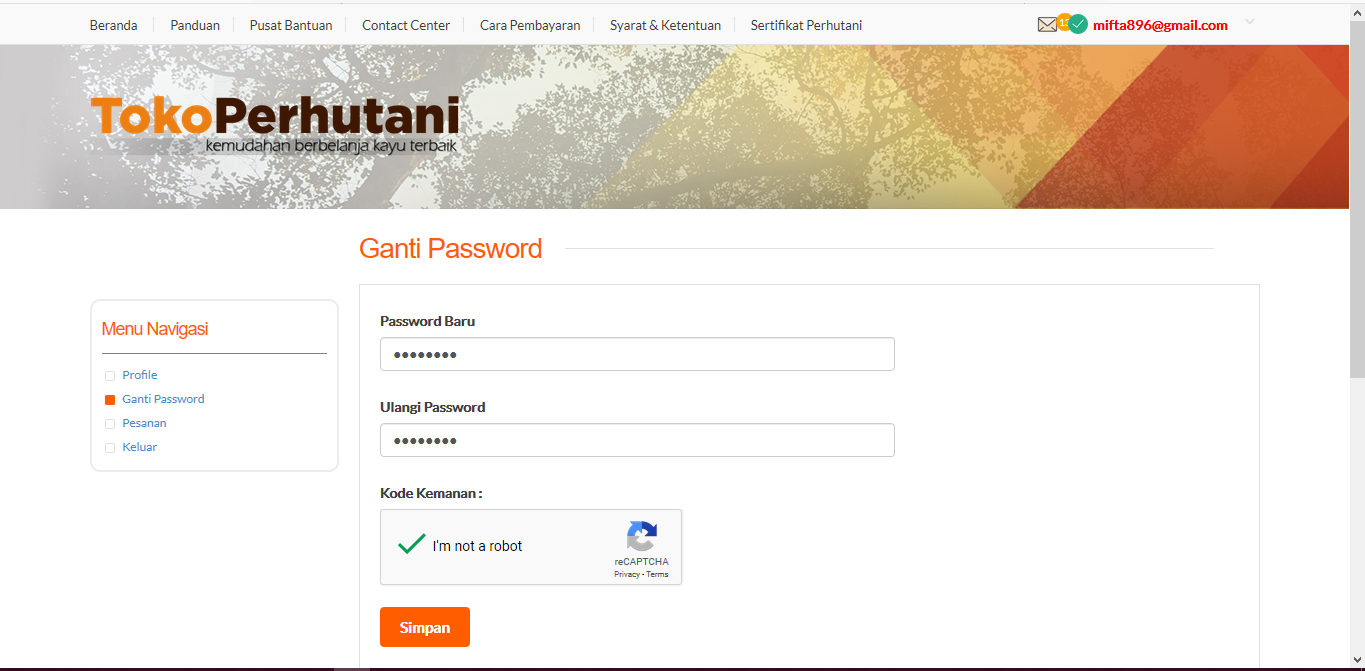
\includegraphics[scale=0.25]{figures/3GantiPassword}
	\caption{Halaman Reset Password}
\end{figure}

\newpage
\subsection{Contact Center WA}
Berikut ini adalah tutorial untuk menghubungi contact center WA. Setelah Login dan Reset Password kita masuk lagi ke halaman utama dengan kode di bawah ini:

\lstinputlisting[language=Python, firstline=38, lastline=38, caption=Halaman Beranda]{src/dinda.py}

Hasilnya  di Google Chrome Akan masuk di halaman beranda seperti ini : 

\begin{figure}[h]
	\centering
	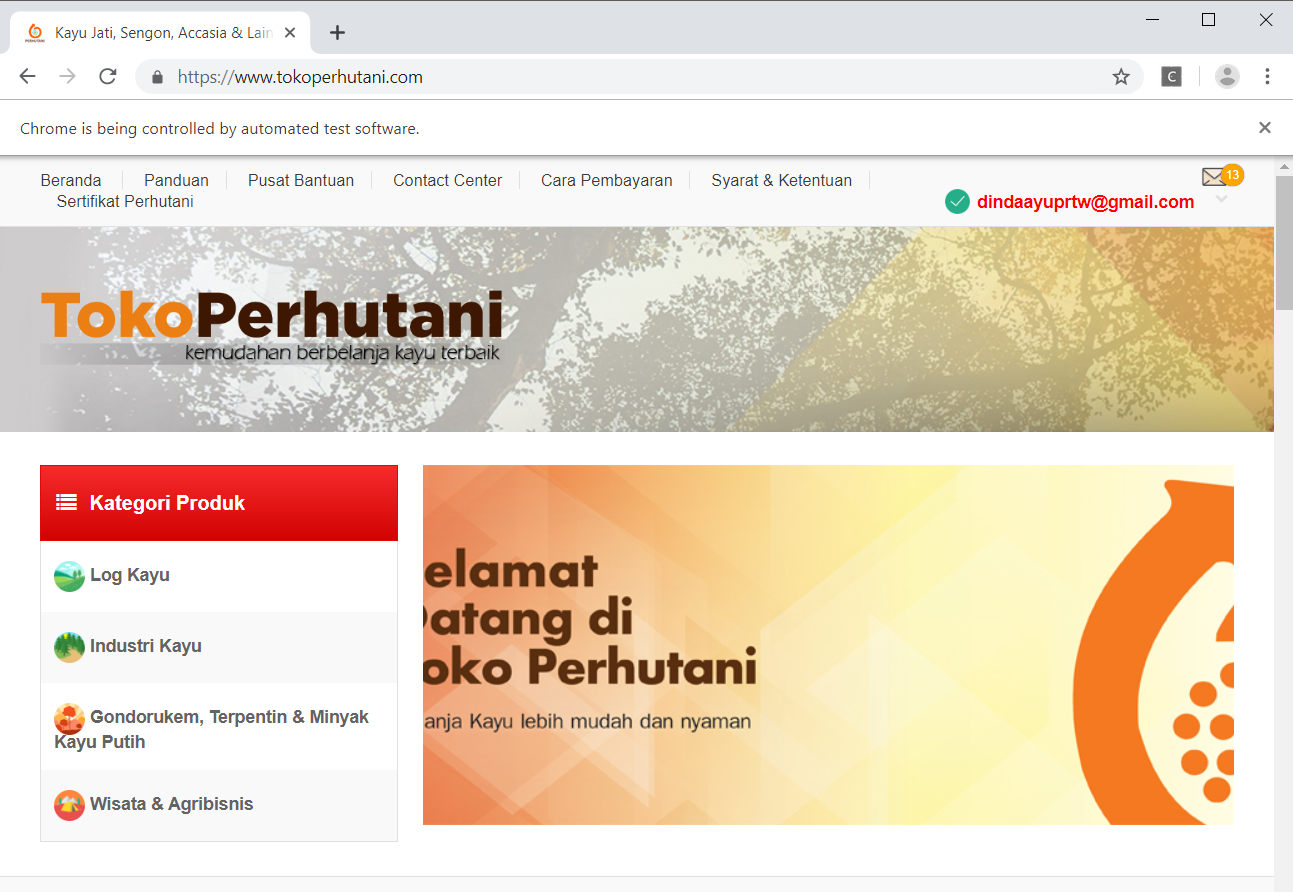
\includegraphics[scale=0.28]{figures/3HalUtama}
	\caption{Halaman Utama/Beranda}
\end{figure}

Masukkan code berikut untuk test masuk menu contact center dengan mencari link text Contact Center:

\lstinputlisting[language=Python, firstline=39, lastline=39, caption=Halaman Contact Center]{src/dinda.py}

Hasilnya  di Google Chrome Akan masuk di halaman contact center seperti ini : 

\begin{figure}[h]
	\centering
	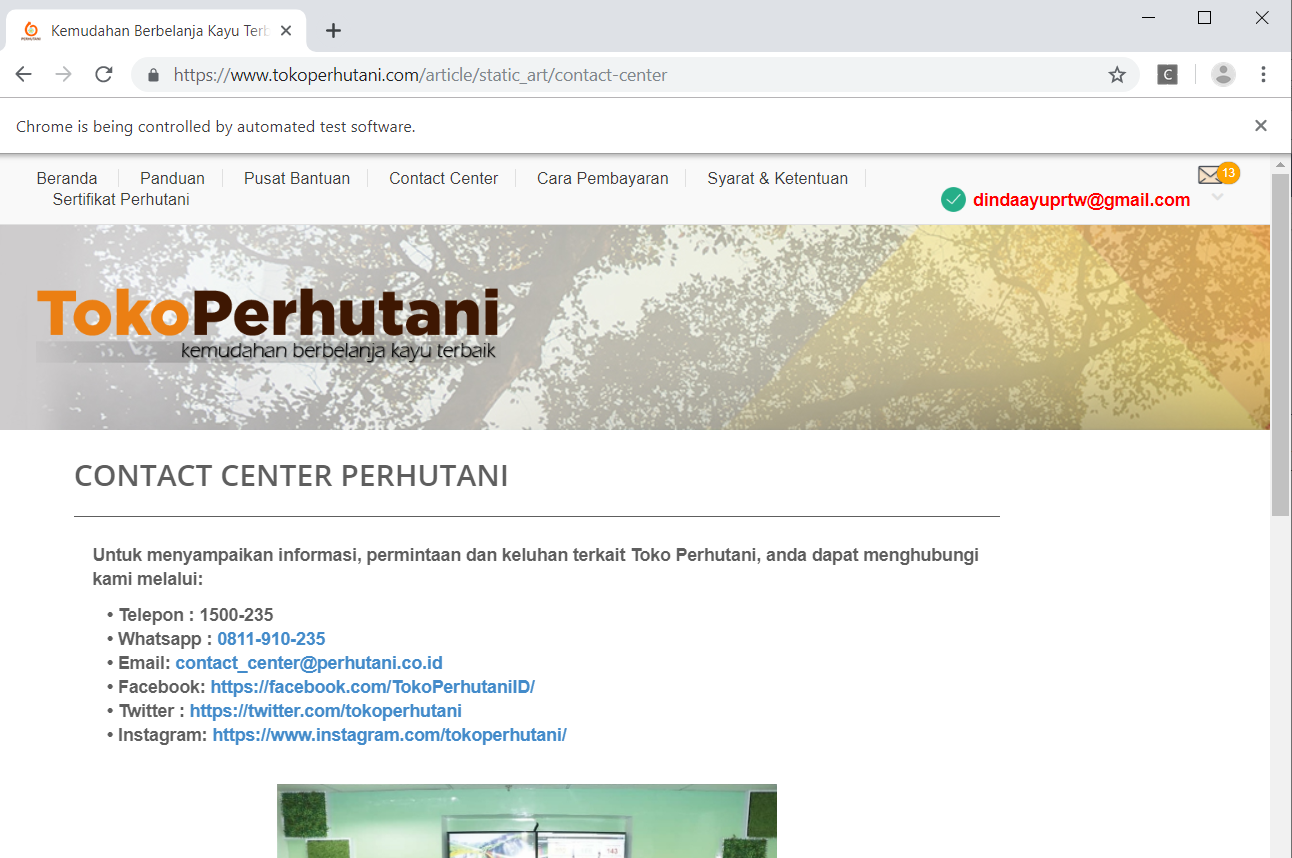
\includegraphics[scale=0.27]{figures/5kontak}
	\caption{Halaman Contact Center}
\end{figure}

Masukkan code berikut untuk test link kontak wa:

\lstinputlisting[language=Python, firstline=40, lastline=40, caption=Halaman Whatsdinda]{src/dinda.py}

Hasilnya  di Google Chrome Akan masuk di halaman whatsdinda : 

\begin{figure}[h]
	\centering
	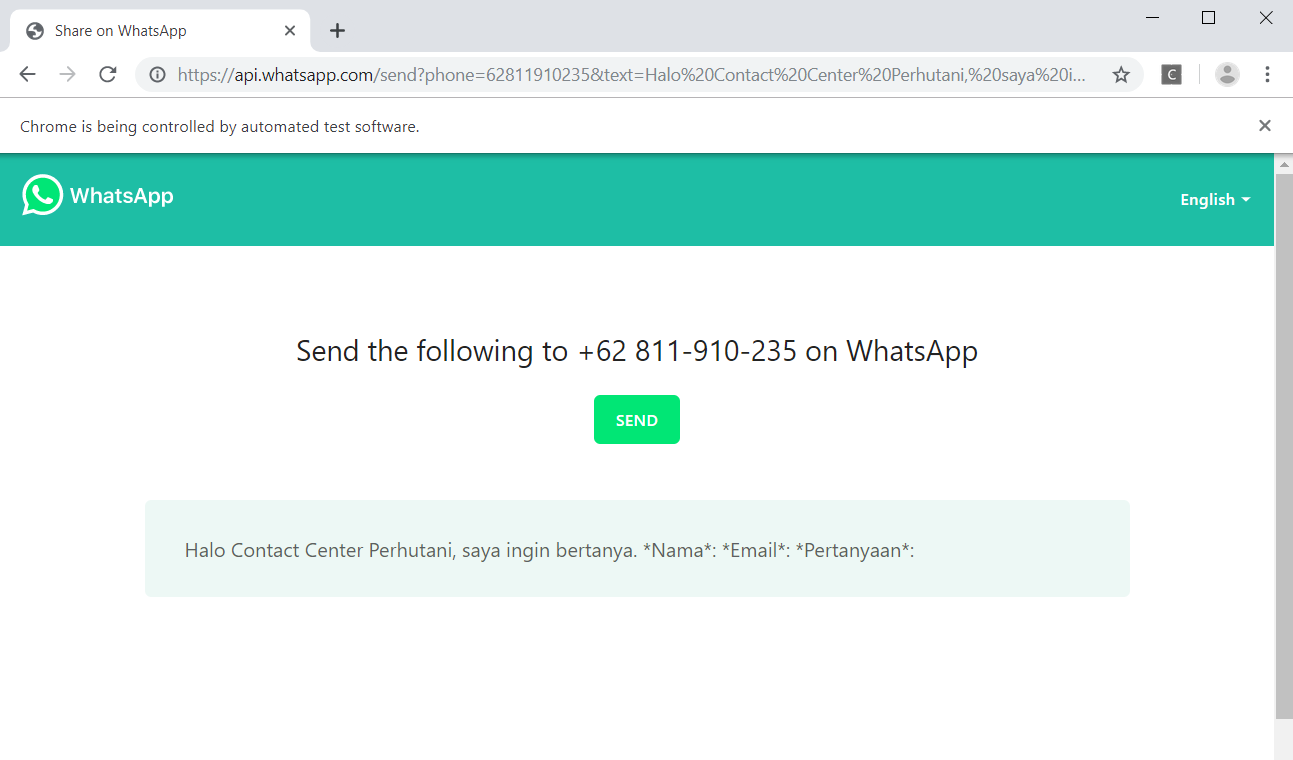
\includegraphics[scale=0.30]{figures/5linkwa}
	\caption{Halaman Whatsdinda}
\end{figure}

\newpage
\section{Cara Login Dan Melihat NIK KTP Pada Profil}
Kali ini kita akan membuat langkah-langkah untuk masuk ke akun tokoperhutani.com dan melihat nik KTP pada menu profil.  
\subsection{Tutorial Login}
Untuk login pada akun tokoperhutani.com masukkan kode berikut pada tool Spyder:
\begin{verbatim}
browser.find_element_by_xpath('/html/body/div
/nav/div/div[2]/ul/li[1]/a/strong').click()
browser.find_element_by_id('email').send_keys
('novinurinabb25@gmail.com')
browser.find_element_by_id('password').send_k
eys("86083F")
browser.find_element_by_class_name('le-button
').click()
\end{verbatim}

Penjelasan:
\begin{enumerate}
	\item Baris pertama untuk mengklik menu login agar form login terbuka.
	\item Baris Kedua untuk mengisikan email pada form login. 
	\item Baris Ketiga untuk mengisi password pada form login.
	\item Baris Keempat untuk mengklik tombol login agar bisa login ke akun yang di inputkan di email dan password.
\end{enumerate}

\newpage
\subsection{Mencari NIK KTP Pada Profil}
Untuk mencari dan menemukan NIK KTP pada profil, masukkan code berikut :
\begin{verbatim}
browser.find_element_by_xpath('/html/body/div/nav/div/div[2]
/ul/strong/li/a').click()
browser.find_element_by_link_text('Profile').click()
\end{verbatim}

Penjelasan:
\begin{enumerate}
	\item Baris Pertama untuk menampilkan menu pada bar
	\item Baris Kedua untuk meng-klik profil dan menampilkan data dan di dalamnya terdapat NIK
\end{enumerate}

Hasil dari menjalankan code baris ke 1:
\begin{figure}[h]
	\centering
	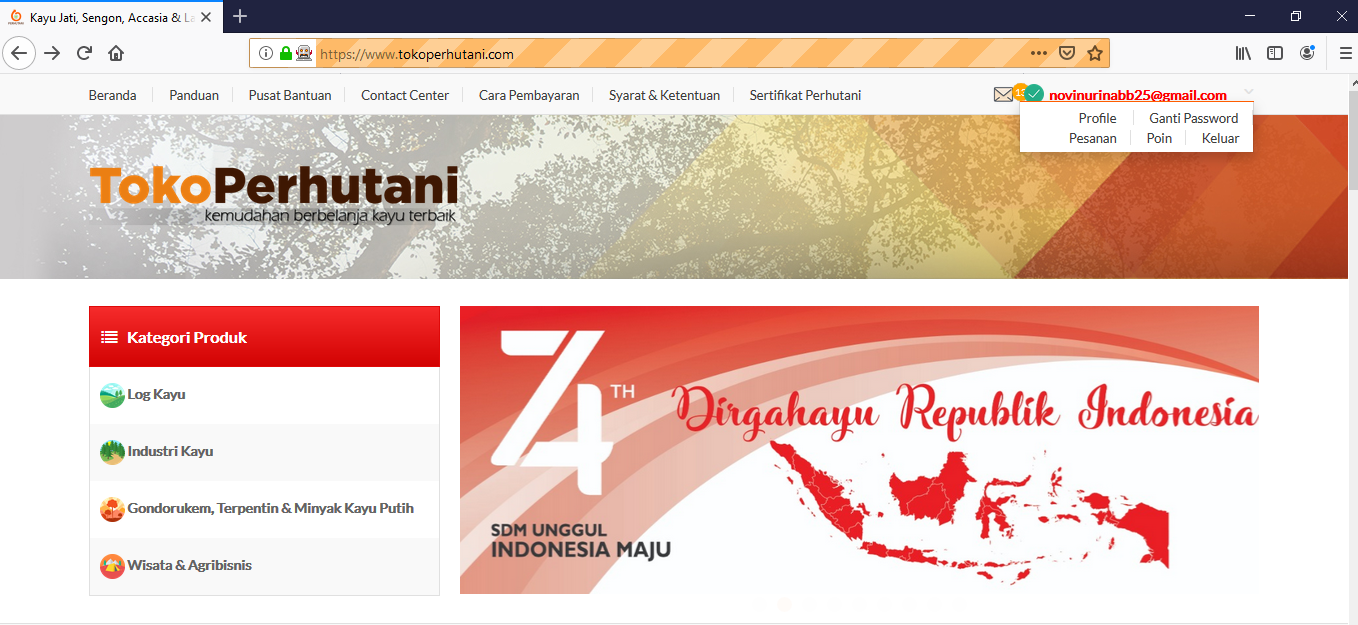
\includegraphics[scale=0.25]{figures/caripropil}
	\caption{Menampilkan Menu Bar Profil}
\end{figure}

Hasil menjalankan code baris ke 2:
\begin{figure}[h]
	\centering
	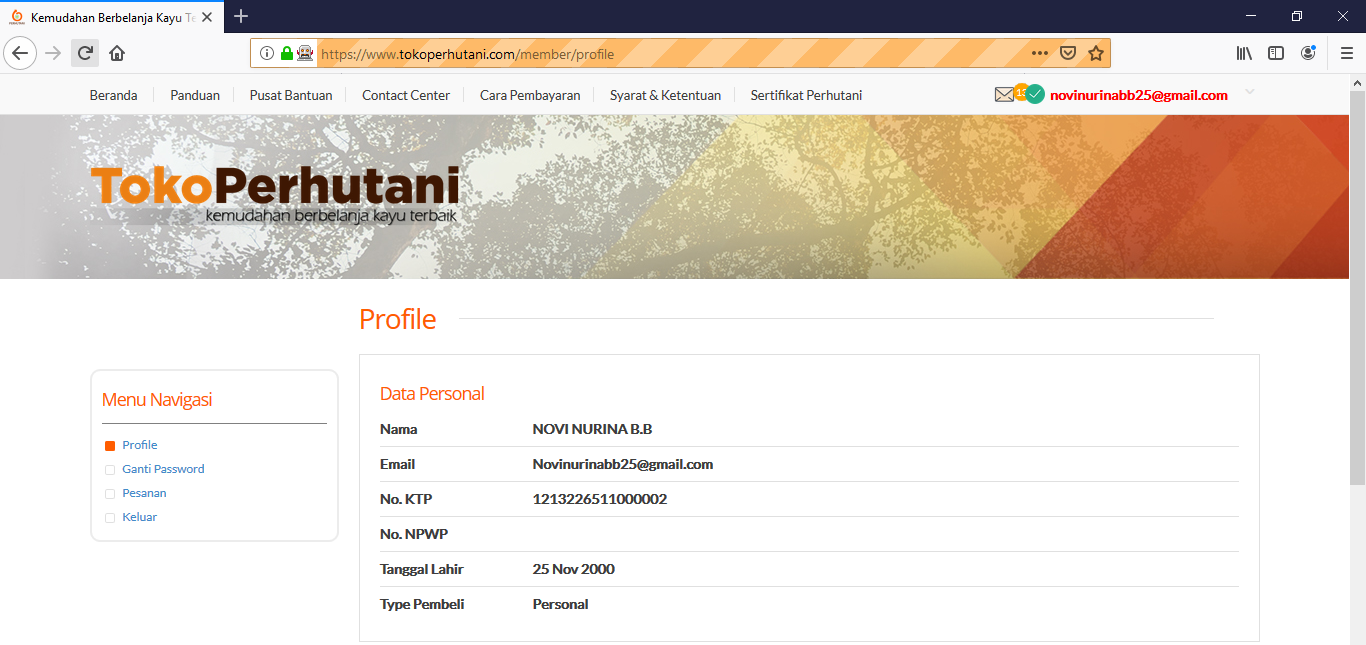
\includegraphics[scale=0.25]{figures/cari}
	\caption{Halaman Profil}
\end{figure}

\newpage
\subsection{Tutorial Login 2}
Untuk login pada akun tokoperhutani.com kita memerlukan informasi akun seperti email dan password lalu masukkan code berikut:
\lstinputlisting[language=Python, firstline=43, lastline=53, caption=Login]{src/dinda.py}

Penjelasan :
\begin{enumerate}
	\item Baris pertama untuk membuka halaman utama toko perhutani
	\item Baris kedua untuk mengklik tombol X pada modal
	\item Baris ketiga untuk mengklik menu login agar form login terbuka
	\item Baris Keempat untuk mengisikan email pada form login 
	\item Baris Kelima untuk mengisi password pada form login
	\item Baris Keenam untuk mengklik tombol login agar bisa login ke akun.
\end{enumerate}

\newpage
Proses login akan berjalan seperti berikut:
\begin{figure}[h]
	\centering
	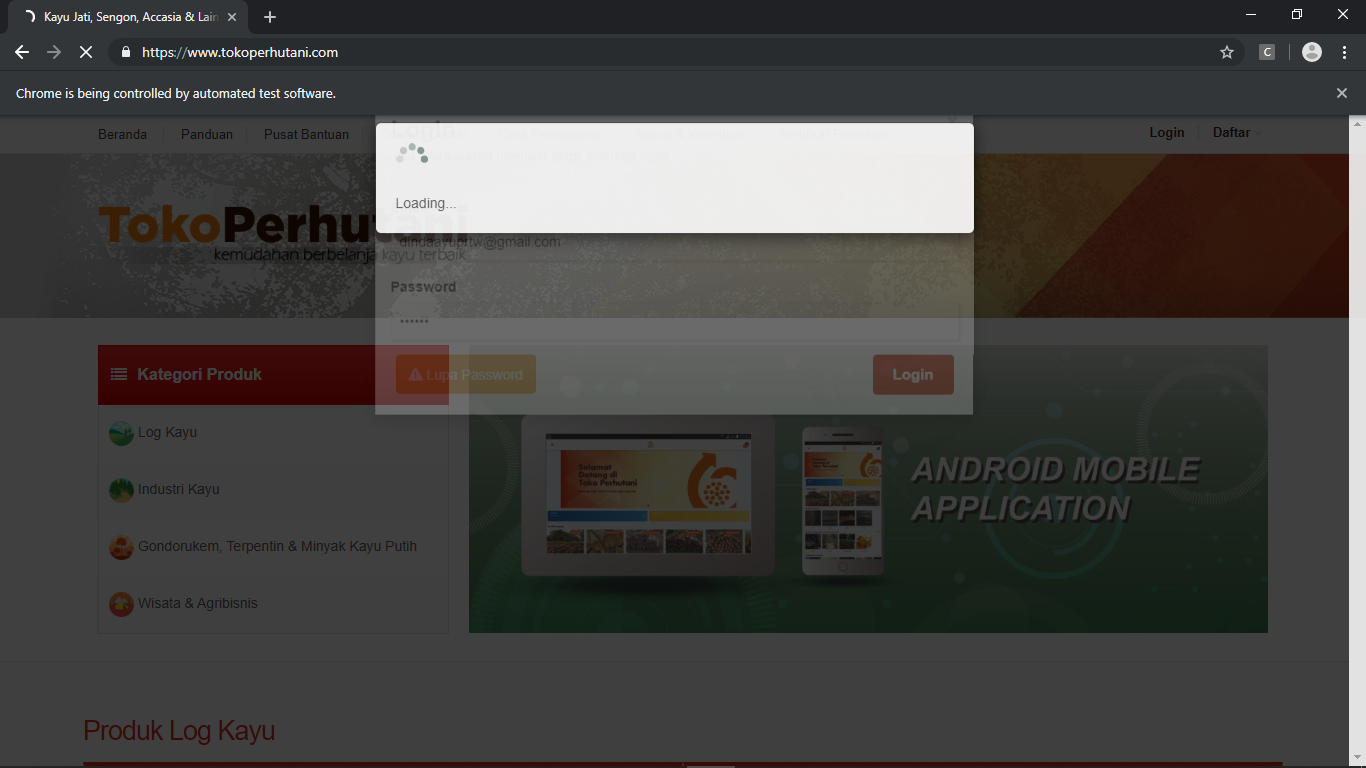
\includegraphics[scale=0.28]{figures/1login}
	\caption{Proses Login}
\end{figure}

Jika login berhasil maka hasilnya akan seperti ini :
\begin{figure}[h]
	\centering
	\includegraphics[scale=0.28]{figures/loginn}
	\caption{Login Berhasil}
\end{figure}

\newpage
\subsection{Menemukan NIK KTP pada Halaman Profil 2}
Untuk menemukan NIK KTP kita harus masuk ke halaman profil dengan masukkan code berikut :
\lstinputlisting[language=Python, firstline=56, lastline=58, caption=Halaman Profile]{src/dinda.py}

Penjelasan :
\begin{enumerate}
	\item Code pada baris pertama berfungsi untuk menampilkan menu pada menu dropdown 
	\item Code pada baris kedua berfungsi untuk mengklik link profile lalu berpindah ke halaman profile.
\end{enumerate}

Hasil dari code baris ke 1 :
\begin{figure}[h]
	\centering
	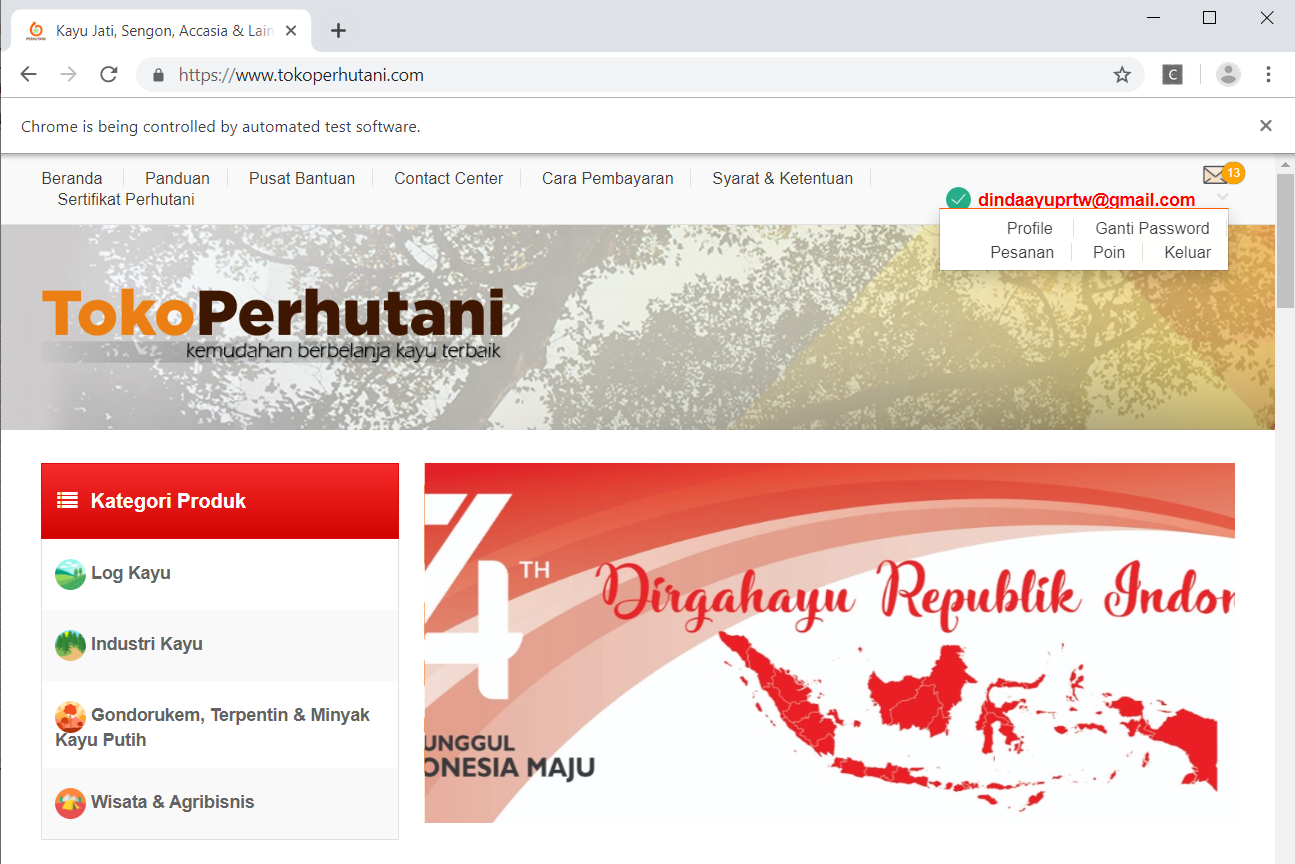
\includegraphics[scale=0.3]{figures/6menubar}
	\caption{Menampilkan Menu Bar Profile}
\end{figure}
\newpage
Hasil dari code baris ke 2:
\begin{figure}[h]
	\centering
	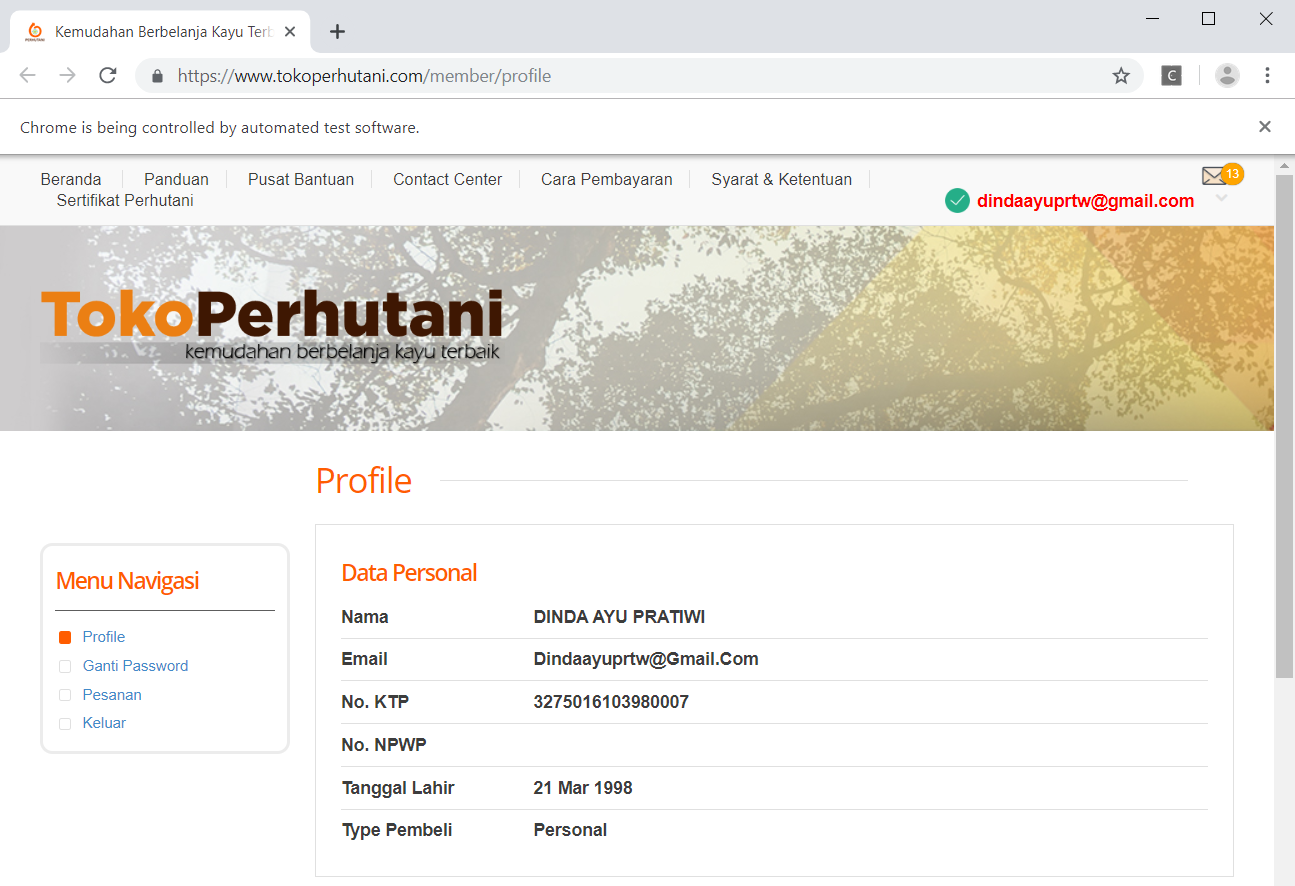
\includegraphics[scale=0.25]{figures/6profile}
	\caption{Halaman Profile}
\end{figure}

Selain menggunakan cara diatas kita dapat langsung masuk ke halaman profile dengan kode berikut:

\lstinputlisting[language=Python, firstline=60, lastline=60, caption=Halaman Profile]{src/dinda.py}

Penjelasan: 
\begin{enumerate}
	\item Kode tersebut akan membuka halaman profile tanpa harus melewati menu 
\end{enumerate}

Setelah kode tersebut dijalankan maka kita akan berada pada halaman profile dan menemukan data diri dan NIK kita seperti berikut:

\begin{figure}[h]
	\centering
	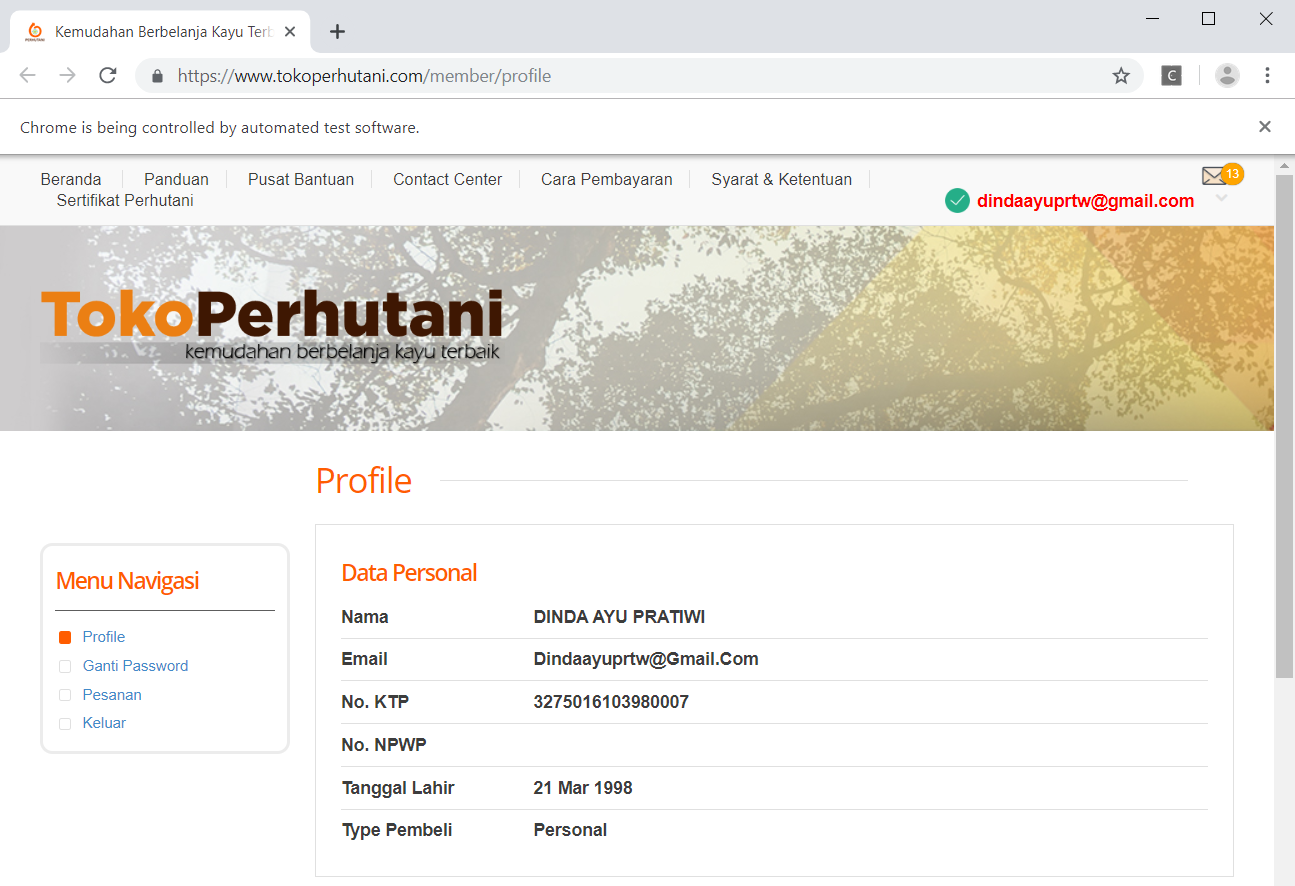
\includegraphics[scale=0.28]{figures/6profile}
	\caption{Halaman Profile}
\end{figure}


\newpage
\subsection{Tutorial Login 3}
Untuk bisa login pada akun tokoperhutani.com maka kita masukkan code berikut pada tools Spyder :
\begin{verbatim}
browser.find_element_by_xpath('/html/body/div
/nav/div/div[2]/ul/li[1]/a/strong').click()
browser.find_element_by_id('email').send_keys
('mifta896@gmail.com')
browser.find_element_by_id('password').send_k
eys("mifta@22")
browser.find_element_by_class_name('le-button
').click()
\end{verbatim}

Penjelasan :
\begin{enumerate}
	\item Baris pertama untuk mengklik menu login agar form login terbuka
	\item Baris Kedua untuk mengisikan email pada form login 
	\item Baris Ketiga untuk mengisi password pada form login
	\item Baris Keempat untuk mengklik tombol login agar bisa login ke akun yang di inputkan di email dan password.
\end{enumerate}

Jika login berhasil maka hasilnya akan seperti ini :
\begin{figure}[h]
	\centering
	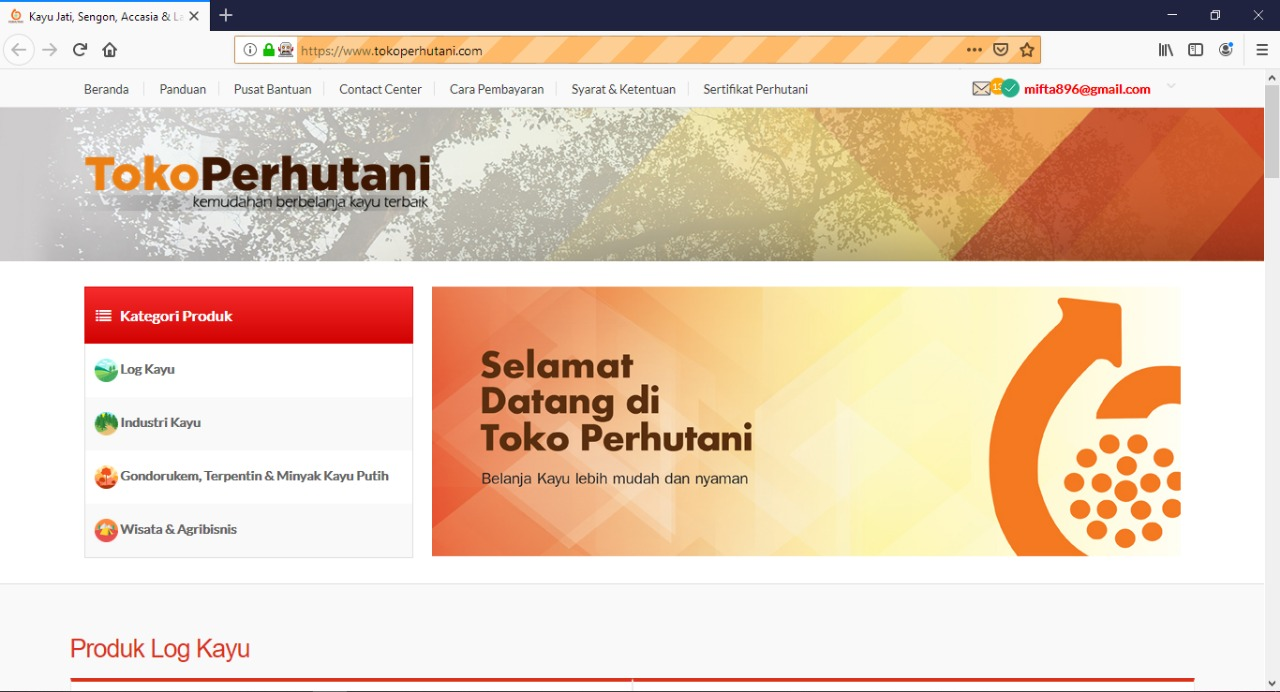
\includegraphics[scale=0.25]{figures/6LOGIN}
	\caption{Login Berhasil}
\end{figure}

\newpage
\subsection{Menemukan NIK KTP Pada Profil 3}
Untuk menemukan NIK KTP pada profil masukkan code berikut :
\begin{verbatim}
browser.find_element_by_xpath('/html/body/div/nav/div/div[2]
/ul/strong/li/a').click()
browser.find_element_by_link_text('Profile').click()
\end{verbatim}

Penjelasan :
\begin{enumerate}
	\item Baris Pertama untuk menampilkan menu pada bar
	\item Baris Kedua untuk mengklik profile dan menampilkan data dan di dalamnya terdapat NIK
\end{enumerate}

Hasil running code baris ke 1 :
\begin{figure}[h]
	\centering
	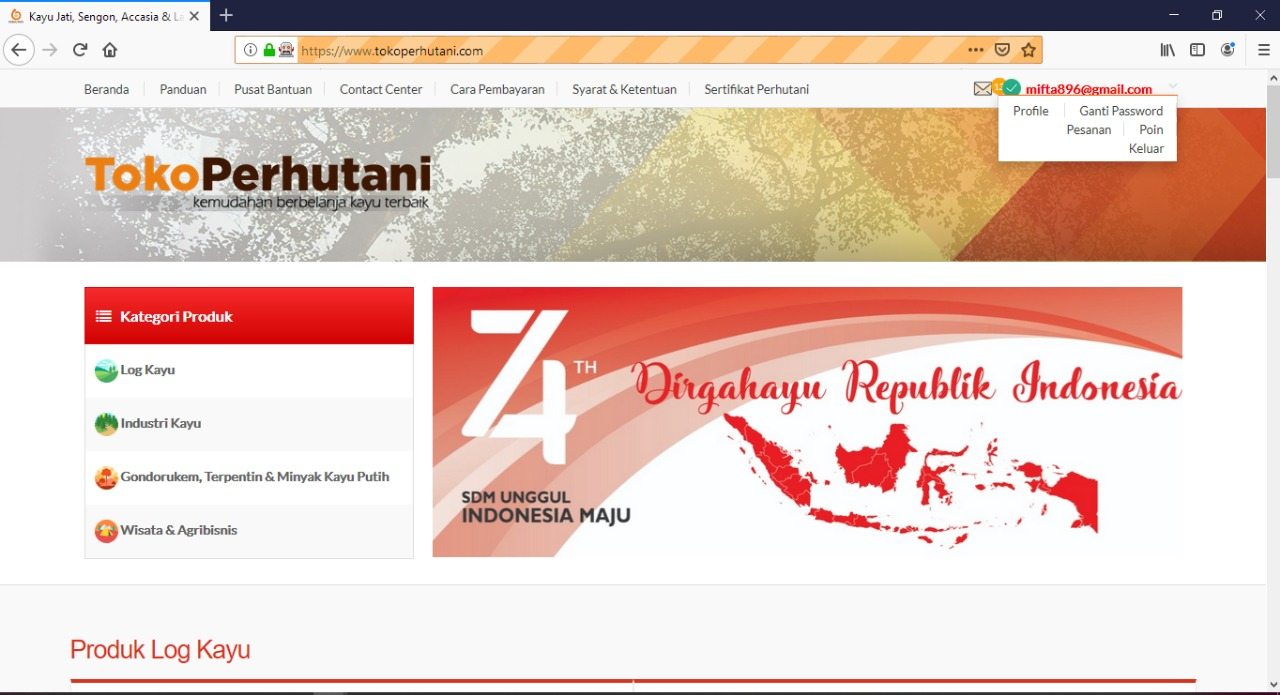
\includegraphics[scale=0.28]{figures/1NIK}
	\caption{Menampilkan Menu Bar Profil}
\end{figure}
\newpage
Hasil running code baris ke 2:
\begin{figure}[h]
	\centering
	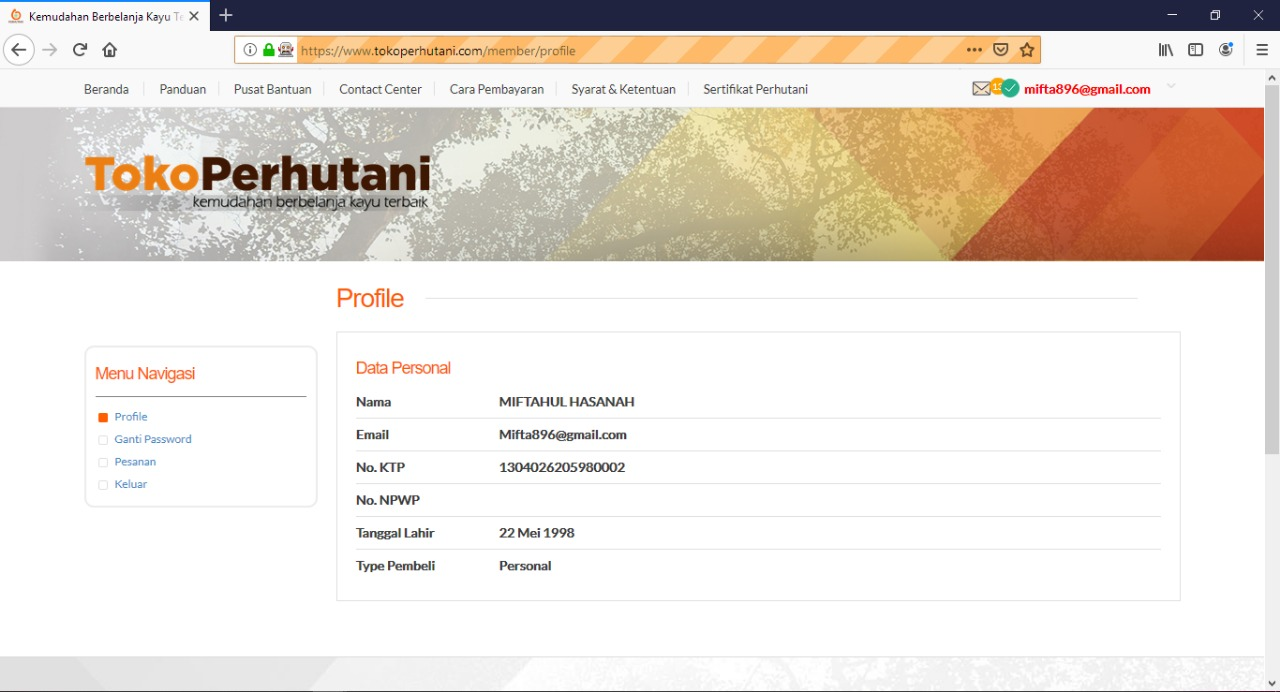
\includegraphics[scale=0.25]{figures/2NIK}
	\caption{Halaman Profil}
\end{figure}


\subsection {Menemukan NIK KTP pada Menu Profil 4}
Untuk menemukan NIK KTP pada profil, masukkan code berikut :
\begin{verbatim}
browser.find_element_by_xpath('/html/body/div/nav/div/div[2]
/ul/strong/li/a').click()
browser.find_element_by_link_text('Profile').click()
\end{verbatim}

Maka akan menjalankan kode dari baris ke 1:
\begin{figure}[h]
	\centering
	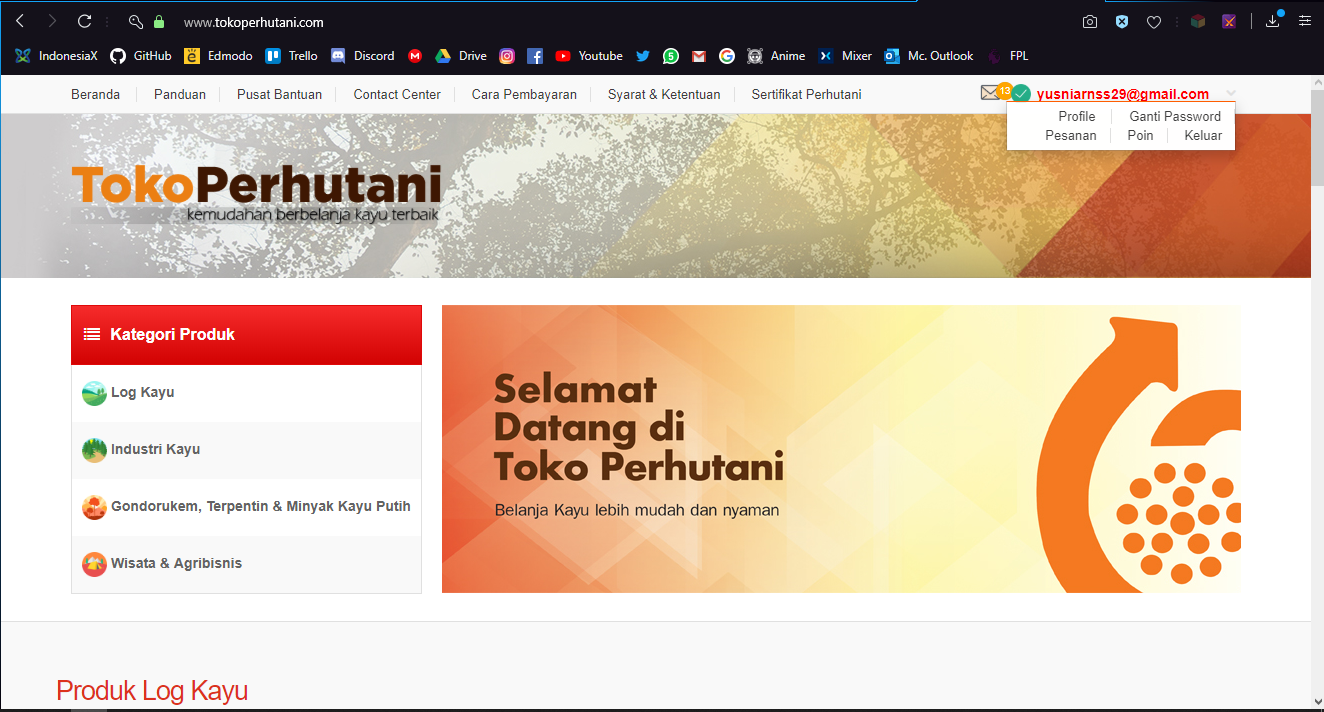
\includegraphics[scale=0.25]{figures/735menuprofile}
	\caption{Menu Bar Profil}
\end{figure}
\newpage
Maka akan menjalankan kode baris ke 2:
\begin{figure}[h]
	\centering
	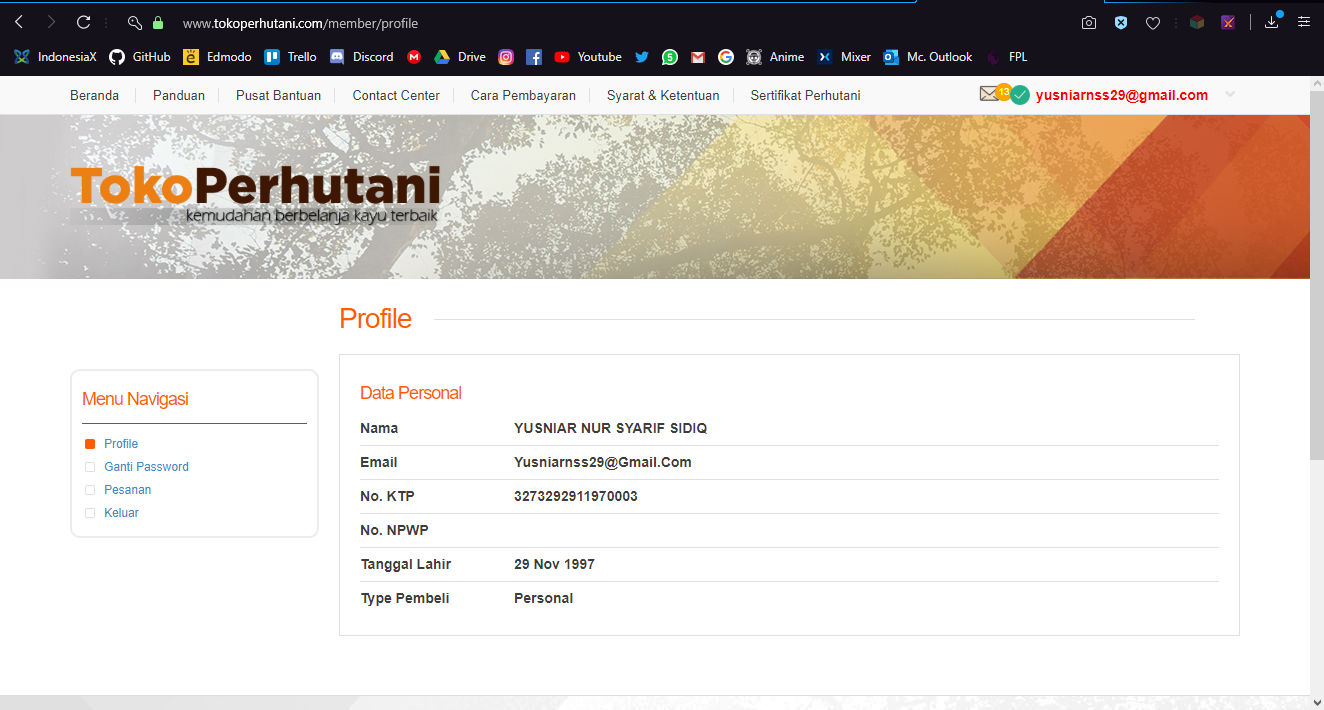
\includegraphics[scale=0.25]{figures/735profilektp}
	\caption{Halaman Profil}
\end{figure}

\newpage
\section{Tutorial Mencari Jenis Kayu Jati, Memasukkannya ke Keranjang Pembelian, dan Konfirmasi Pesanan }

\subsection{Tutorial Mencari Jenis Kayu Jati 1}
Berikut adalah tutorial untuk mencari Jenis Kayu Jati Dan memasukkannya ke keranjang. Masukkan code berikut ini pada spyder:
\begin{verbatim}
Code Untuk masuk ke halaman web tokoperhutani.com :
from selenium import webdriver
opsi = webdriver.firefox.options.Options()
opsi.headless = False
binary = webdriver.firefox.firefox_binary.FirefoxBinary
('C:\\Program Files\\Mozilla Firefox\\firefox.exe')
cap = webdriver.common.desired_capabilities.Desired
Capabilities().FIREFOX
cap['marionette'] = True
browser=webdriver.Firefox(options=opsi,capabi
lities=cap,firefox_binary=binary)
browser.get('https://tokoperhutani.com/')
pemberitahuan = browser.find_element_by_xpath('//*[@id="
bannerModal"]/div/div/div[1]/button').click()
retail = browser.get('https://tokoperhutani.
com/beranda')

Code untuk login di web tokoperhutani.com :
login = browser.find_element_by_xpath('/html/body/
div/nav/div/div[2]/ul/li[1]/a/strong').click()
email = browser.find_element_by_id('email').send_
keys('novinurinabb25@gmail.com')
password = browser.find_element_by_id('password').
send_keys("86083F")
tombol = browser.find_element_by_class_name
('le-button').click()
browser.find_element_by_link_text('Beranda')
.click()

Code untuk memilih jenis kayu jati :
retail = browser.get('https://tokoperhutani.com/beranda')
wilayah = browser.find_element_by_id
('wilayah').click()
plh_wilayah = browser.find_element_by_xpath('//*[@id="wilayah"]
/option[4]').click()
kota = browser.find_element_by_id('kota').
click()
plh_kota = browser.find_element_by_xpath
('//*[@id="kota"]/option[3]').click()
tpk = browser.find_element_by_id
('select_kota').click()
plh_tpk = browser.find_element_by_xpath
('//*[@id="select_kota"]/option[3]').click()
cari = browser.find_element_by_id('i_submit').
click()
\end{verbatim}

Berikut hasil running dari code :
\begin{figure}[h]
	\centering
	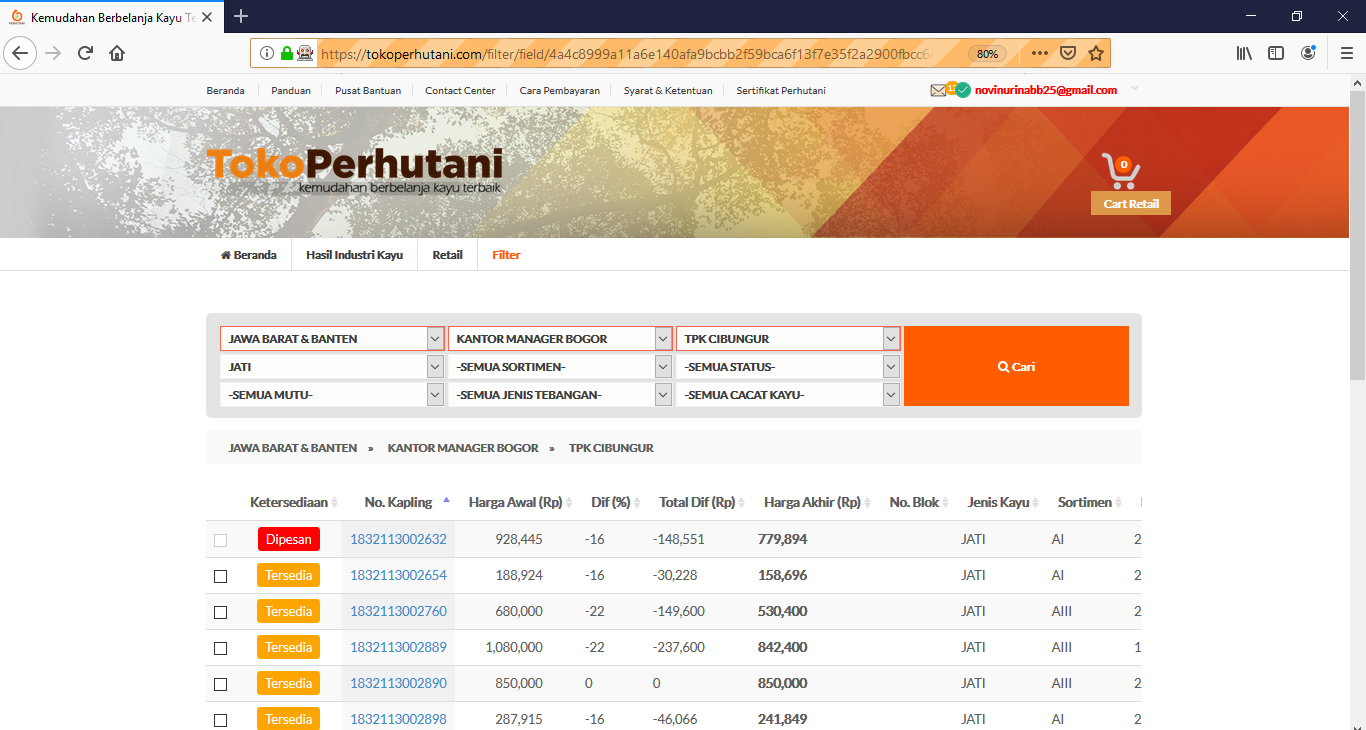
\includegraphics[scale=0.25]{figures/jatii}
	\caption{Mencari Kayu Jati}
\end{figure}

Kemudian masukkan code ini untuk memasukkan kayu jati ke dalan keranjang :
\begin{verbatim}
beli_sekarang = browser.find_element_by_xpath('/html
/body/div/strong/div[8]/div/div/form/input').click()
\end{verbatim}
Hasil dari code adalah sebagai berikut :
\begin{figure}[h]
	\centering
	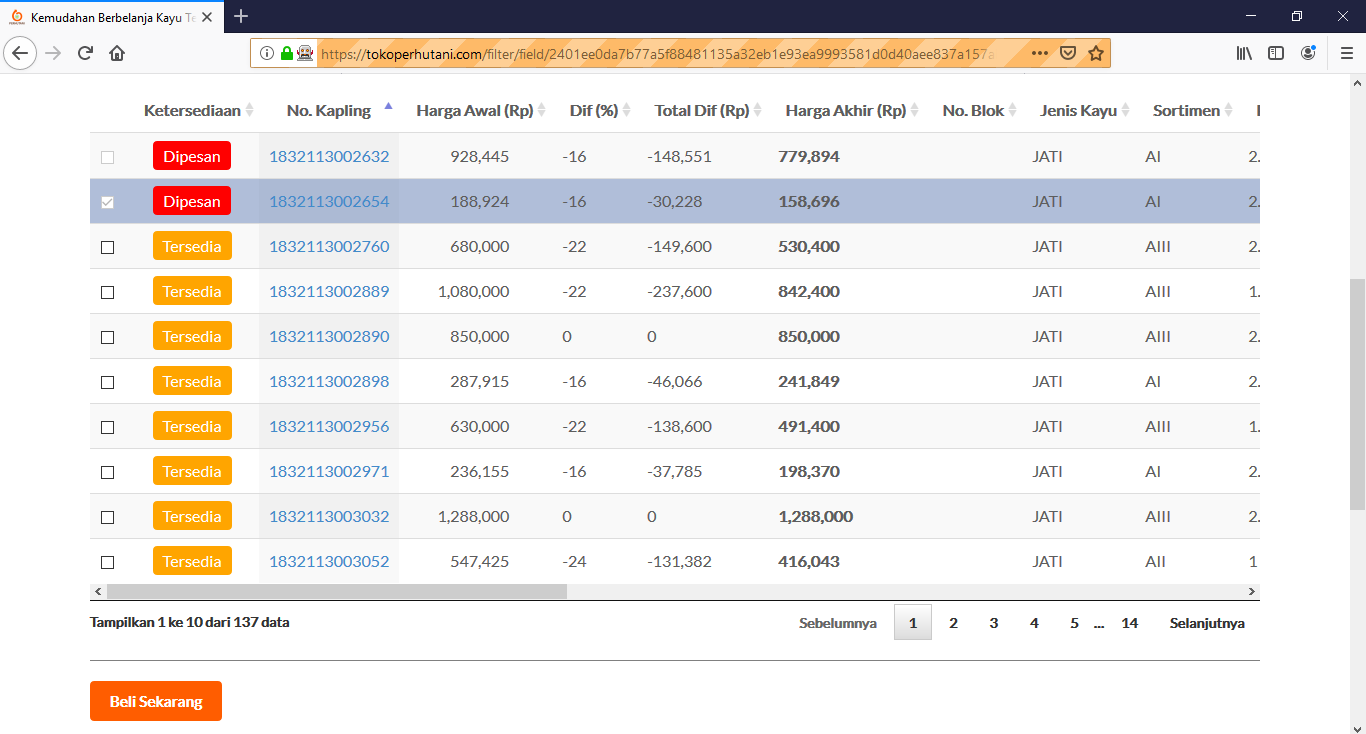
\includegraphics[scale=0.25]{figures/belii}
	\caption{Beli Kayu Jati}
\end{figure}

\newpage
Tekan beli sekarang maka otomatis barang akan masuk ke dalam keranjang belanja :
\begin{figure}[h]
	\centering
	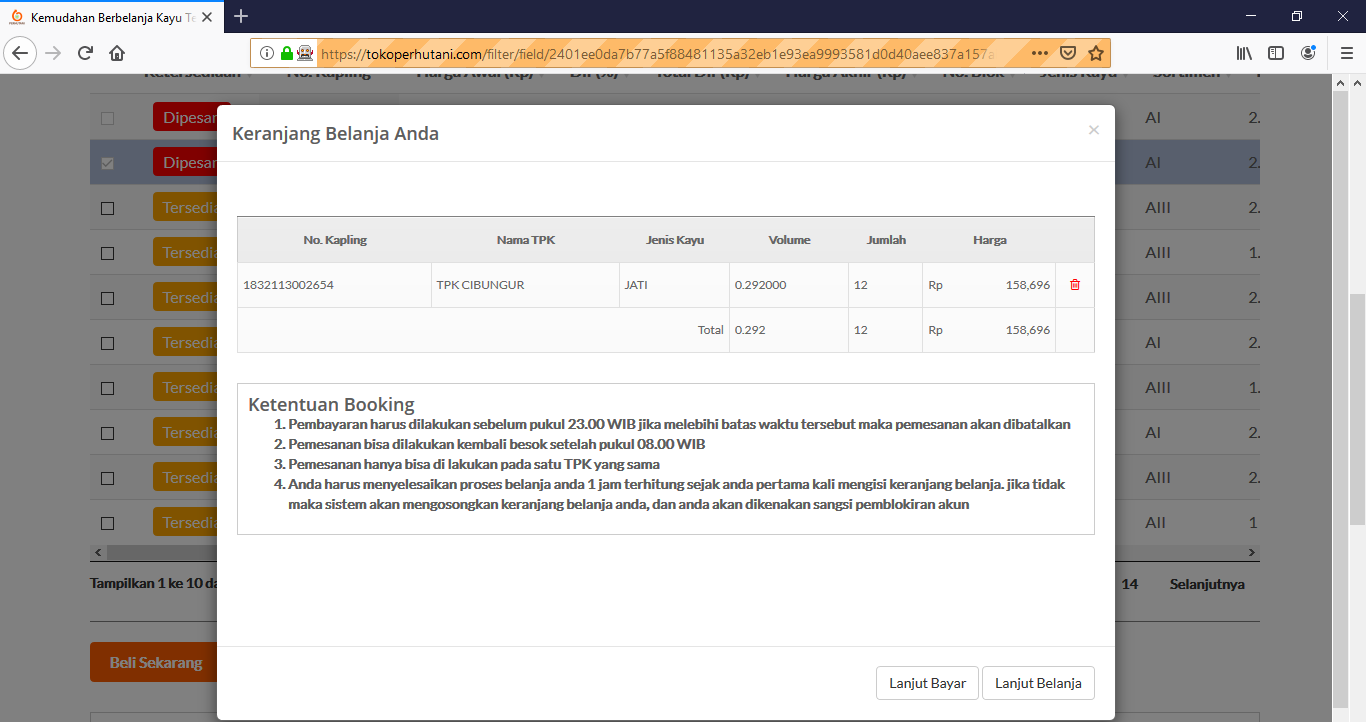
\includegraphics[scale=0.25]{figures/keranjangg}
	\caption{Barang Masuk Ke Keranjang}
\end{figure}

\subsection{Konfirmasi Pesanan 1}
Tutorial selanjutnya yaitu konfirmasi pesanan hingga menerima email pesanan. 
Masukkan code berikut pada spyder :
\begin{verbatim}
lanjut_belanja = browser.find_element_by_xpath('/html
/body/div[1]/strong/div[5]/div/div/div[3]/a/button').
click()
bank_bri = browser.find_element_by_xpath('/
html/body/div/strong/section[2]/div/div[2]/
div/div/form/div/ul/li[2]/label/img').click()
\end{verbatim}

Berikut hasil debug dari code :
\begin{figure}[h]
 	\centering
 	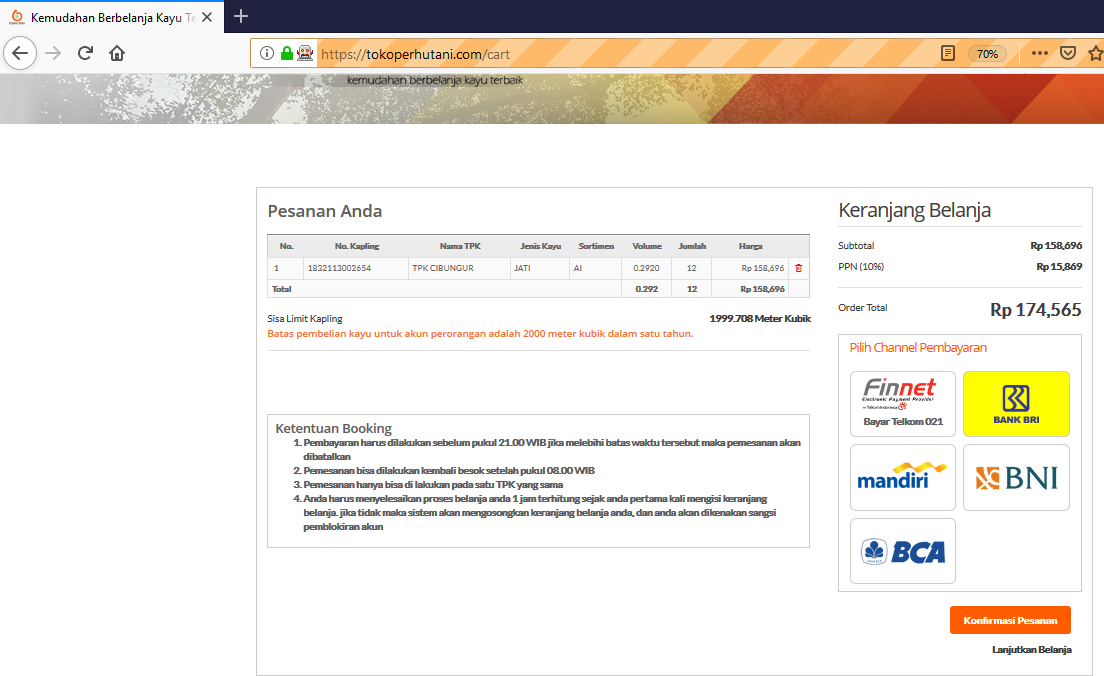
\includegraphics[scale=0.26]{figures/bayar}
 	\caption{Konfirmasi Pembayaran}
\end{figure}
 
Kemudian Masukkan code berikut untuk melanjutkan proses:
\begin{verbatim}
konfirmasi_pemesanan = browser.find_element_by_xpath('//*
[@id="confirmOrder"]')
\end{verbatim}
Berikut hasil debug dari code: 
\begin{figure}[h]
	\centering
	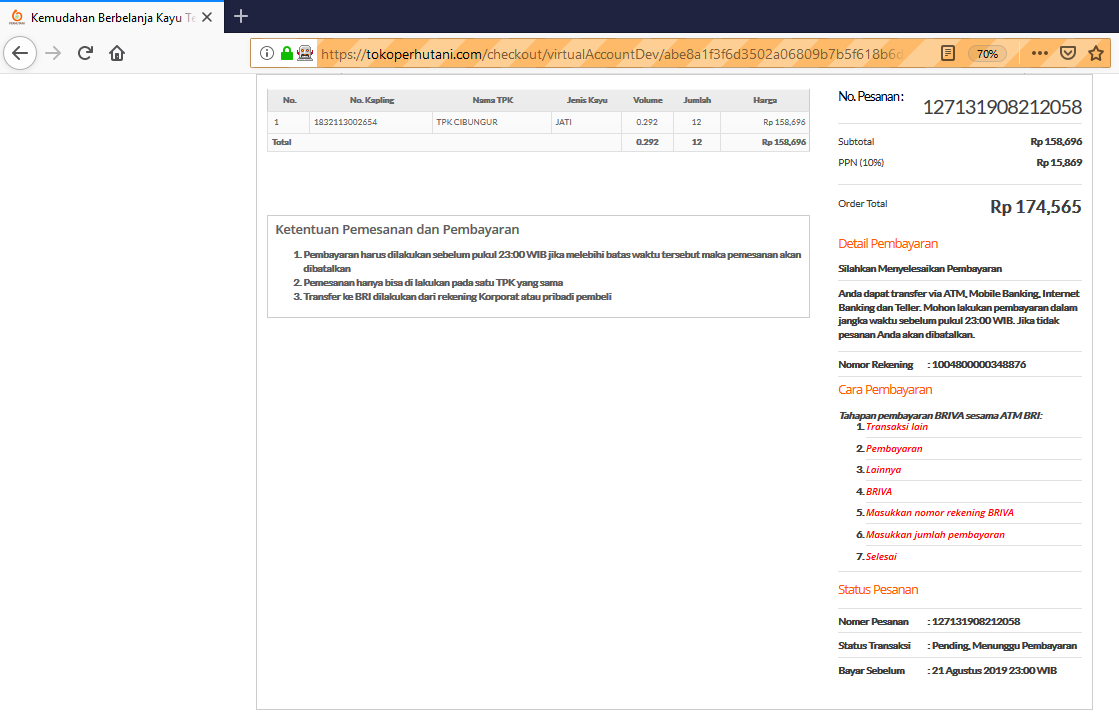
\includegraphics[scale=0.25]{figures/invoicee}
	\caption{Invoice Pembayaran}
\end{figure}

Jika proses berhasil akan masuk pesan ke email kita seperti tampilan berikut:
\begin{figure}[h]
	\centering
	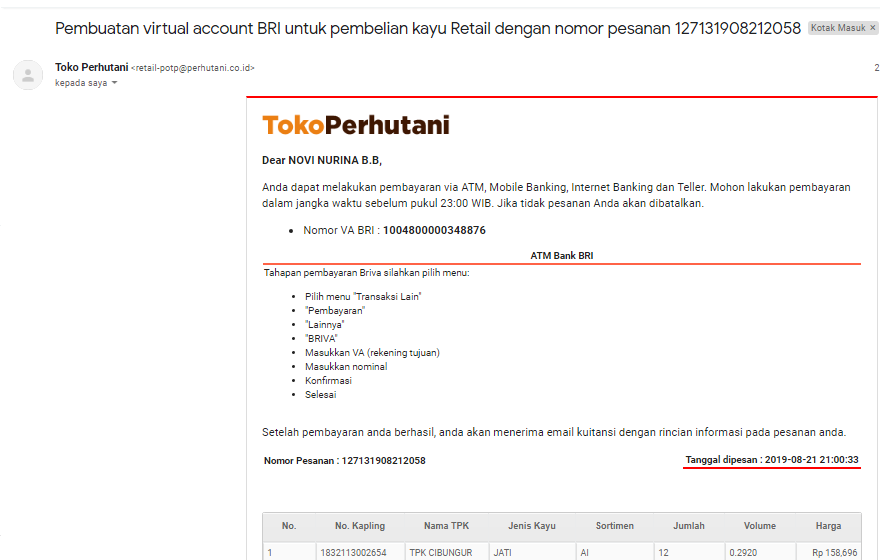
\includegraphics[scale=0.30]{figures/emailbayar}
	\caption{Pesan Email}
\end{figure}

\newpage
\subsection {Tutorial Mencari Jenis Kayu Jati 2}
Langkah yang perlu dilakukan adalah, masukkan kode berikut di spyder :
\begin{verbatim}
browser=webdriver.Firefox(options=opsi,capabilities=cap,firefox_binary=binary)
browser.get('https://www.tokoperhutani.com/filter/field/c04a3f05d53cdf8f8ac5cf643ba2504bd2f46bd0bb9a60877d640d51d96a6af5#')
\end{verbatim}

Sehingga akan diarahkan ke Pembelian Kayu Jati. Dan langkah berikutya adalah memilih jenis Kayu Jatinya dan memasukkannya kedalam keranjang pembelian. Seperti screenshot di bawah ini.
\begin{figure}[h]
	\centering
	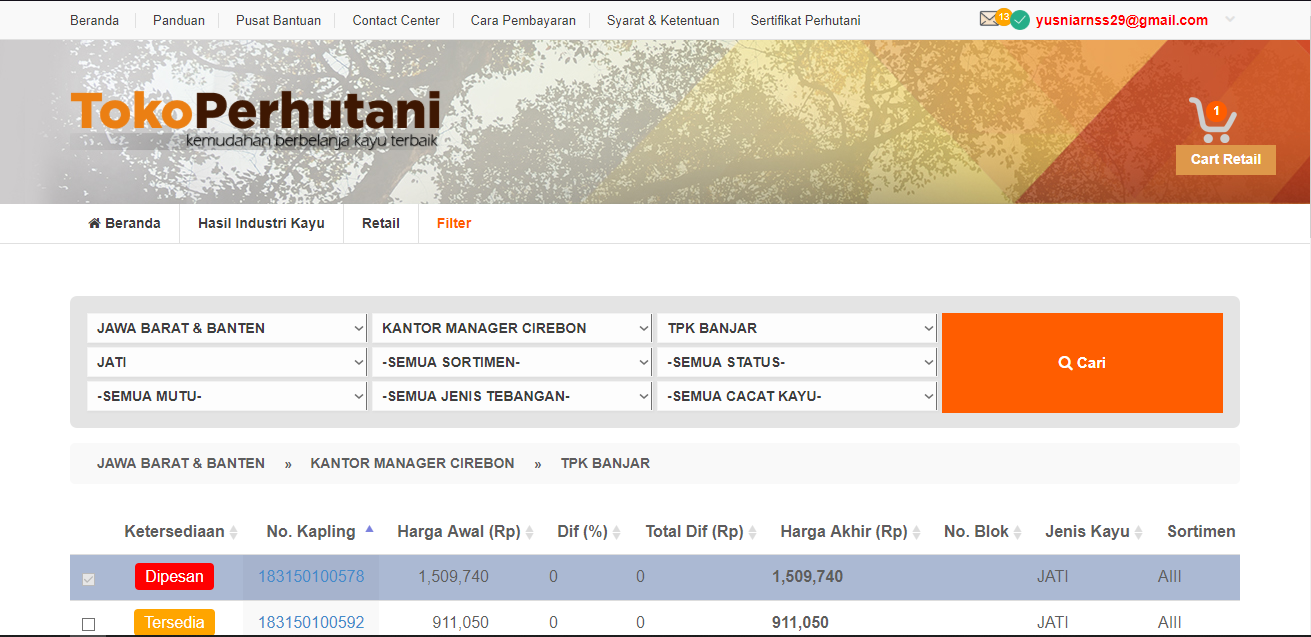
\includegraphics[scale=0.25]{figures/T5_cart}
	\caption{Keranjang Pembelian}
\end{figure}

\newpage
\subsection {Melakukan Konfirmasi Pemesanan 2}
Untuk melakukan konfirmasi Pemesanan, pertama jalankan dahulu kode berikut :
\begin{verbatim}
browser=webdriver.Firefox(options=opsi,capabilities=cap,firefox_binary=binary)
browser.get('https://www.tokoperhutani.com/member/order')
\end{verbatim}

Maka akan diarahkan ke Menu Konfirmasi Pemesanan yang terdapat pada Inbox akun.
Gambar dibawah merupakan konfirmasi pemesanan Kayu Jati:
\begin{figure}[h]
	\centering
	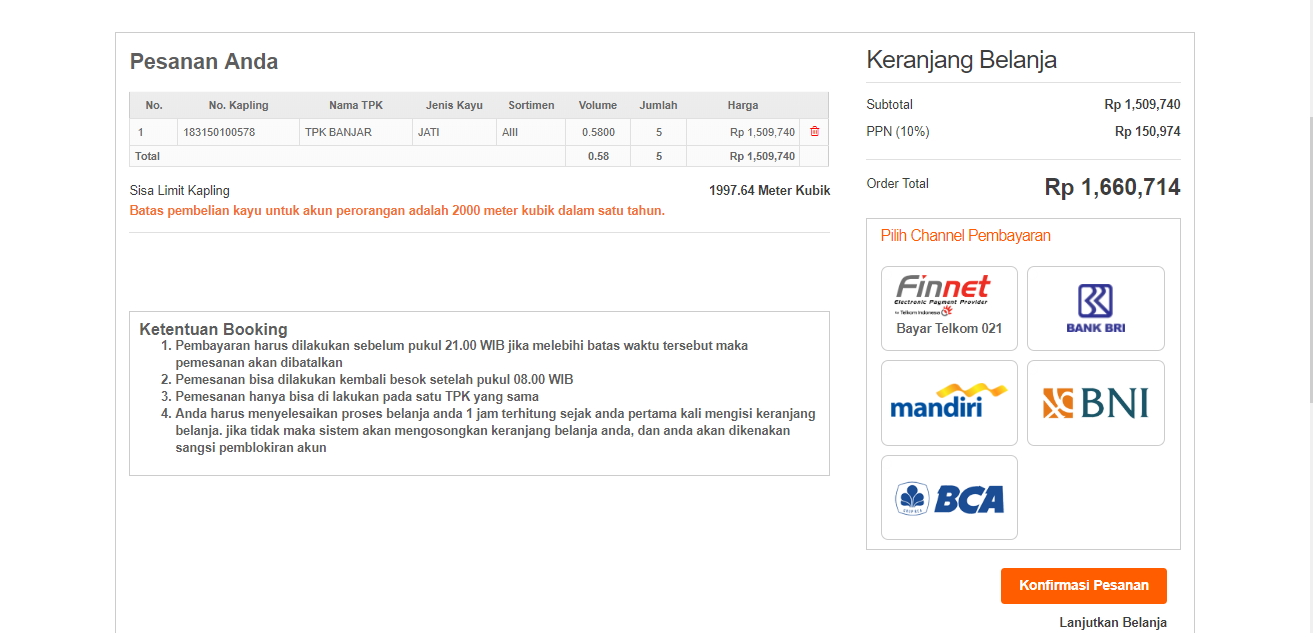
\includegraphics[scale=0.25]{figures/T6_1}
	\caption{Konfirmasi Pemesanan Kayu Jati}
\end{figure}

Gambar dibawah merupakan screenshot untuk
\begin{figure}[h]
	\centering
	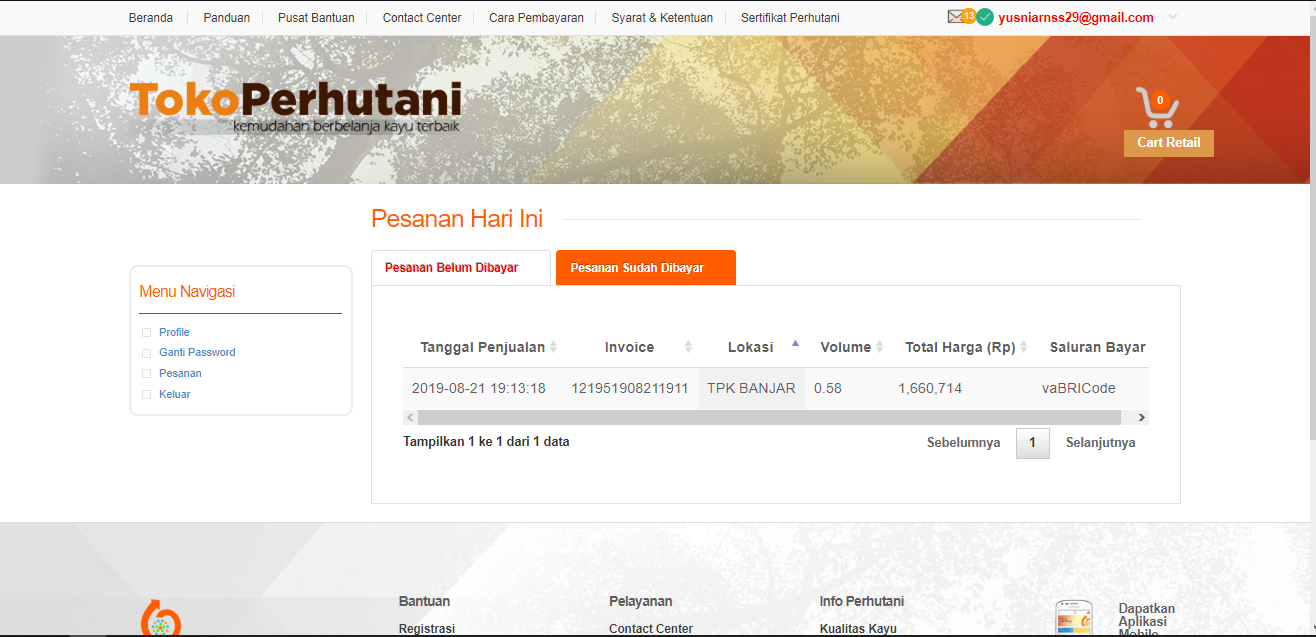
\includegraphics[scale=0.25]{figures/T6_2}
	\caption{Email Pemesanan Kayu Jati}
\end{figure}

\newpage
\subsection{Tutorial Mencari Jenis Kayu Jati 3}
Berikut adalah tutorial untuk mencari Kayu Jati Dan memasukkan ke keranjang. Masukkan code berikut ini pada spyder:
\lstinputlisting[language=Python, firstline=66, lastline=75, caption=Login]{src/dinda.py}

Kode diatas berfungsi untuk masuk ke web toko perhutani dan melakukan login.
Langkah selanjutnya adalah masuk ke beranda dan mencari kayu yang akan dimasukan ke keranjang.

\lstinputlisting[language=Python, firstline=77, lastline=98, caption=Mencari Kayu Jati]{src/dinda.py}

\newpage
Jika kode tersebut berhasil di jalankan maka berikut hasil running dari kode diatas pada tombol ketersediaan akan berubah menjadi dipesan:
\begin{figure}[h]
	\centering
	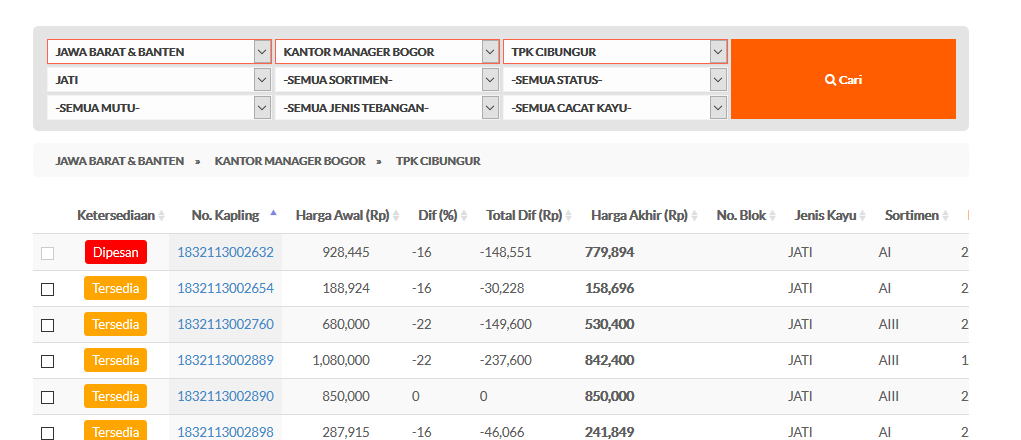
\includegraphics[scale=0.3]{figures/6keranjang}
	\caption{Mencari Kayu Jati}
\end{figure}

Kemudian kode berikut untuk menekan beli sekarang maka otomatis barang akan masuk ke dalam keranjang belanja:
\lstinputlisting[language=Python, firstline=100, lastline=100, caption=Memasukan Pesanan ke Keranjang]{src/dinda.py}

\newpage
\subsection{Konfirmasi Pesanan 3}
Setelah memasukan kayu kedalam keranjang selanjutnya yaitu konfirmasi pesanan hingga menerima email pesanan. 
Masukkan code berikut:
\lstinputlisting[language=Python, firstline=103, lastline=109, caption=Konfirmasi Pesanan]{src/dinda.py}

Kemudian masukkan code berikut ini untuk melanjutkan proses pemesanan:
\lstinputlisting[language=Python, firstline=111, lastline=111, caption=Melanjutkan Proses Pemesanan]{src/dinda.py}

Hasilnya maka akan dialihkan ke halaman invoice berikut ini:
\begin{figure}[h]
	\centering
	\includegraphics[scale=0.30]{figures/6invoice}
	\caption{Pesan Email}
\end{figure}

Jika proses berhasil akan masuk pesan mengenai informasi pembayaran ke email kita.

\newpage 
\subsection{Mencari Jenis kayu Jati Dan Memasukkannya ke keranjang 4}
Berikut adalah cara kita untuk memilih jenis kayu yaitu jenis kayu jati, terlebih dahulu kita masukkan kodingan berikut ini: 
\begin{verbatim}
retail = browser.get('https://tokoperhutani.com/beranda')
wilayah = browser.find_element_by_id('wilayah').click()
plh_wilayah = browser.find_element_by_xpath('//*
[@id="wilayah"]/option[4]').click()
kota = browser.find_element_by_id('kota').click()
plh_kota = browser.find_element_by_xpath('//
*[@id="kota"]/option[3]').click()
tpk = browser.find_element_by_id('select_kota').click()
plh_tpk = browser.find_element_by_xpath('//
*[@id="select_kota"]/option[3]').click()
cari = browser.find_element_by_id('i_submit').click()
ketersediaan = browser.find_element_by_xpath
('/html/body/div/strong/div[8]/div/div/
form/div/div[3]/div[2]/table/tbody/tr[1]
/td[1]/input').click()
\end{verbatim}

Hasil setelah dijalankan adalah : 
\begin{figure}[h]
	\centering
	\includegraphics[scale=0.25]{figures/carikayu1}
	\caption{Halaman hasil pencarian kayu jati}
\end{figure}

\newpage
langkah selanjutnya adalah kita mengklik button beli sekarang sehingga kita akan masuk kedalam keranjang belanja kita , sebelumnya masukkan kodingan berikut ini: 
\begin{verbatim}
beli_sekarang = browser.find_element_by_xpath
('/html/body/div/strong/div[8]/div/div/
form/input').click()
\end{verbatim}

hasilnya setelah dijalankan adalah kita akan masuk kedalam keranjang belanjaan kita.
\begin{figure}[h]
	\centering
	\includegraphics[scale=0.25]{figures/carikayu2}
	\caption{Halaman keranjang belanjaan}
\end{figure}

Selanjutnya adalah kita klik button lanjut bayar lalu kita pilih bank nya BRI lalu konfirmasi pemesanan, dengan memasukkan kodingan berikut ini: 
\begin{verbatim}
lanjut_belanja = browser.find_element_by_xpath
('/html/body/div[1]/strong/div[5]/div/div/
div[3]/a/button').click()
bank_bri     = browser.find_element_by_xpath
('/html/body/div/strong/section[2]/div/div
[2]/div/div/form/div/ul/li[2]/label/img').click()
konfirmasi_pemesanan=browser.find_
element_by_xpath('//*[@id="confirmOrder"]')
\end{verbatim}

\newpage
Maka hasilnya akan sebagai berikut setelah masuk 
ke email masing masing untuk menunggu pembayaran
\begin{figure}[h]
	\centering
	\includegraphics[scale=0.25]{figures/email1}
	\caption{Halaman pemesanan}
\end{figure}

\newpage
\section{Tutorial mengambil data dari tabel kayu yang dijual dan mengambil data dari tabel pesanan}
Berikut adalah tutorial untuk  mengambil data dari tabel kayu yang dijual dan pengambilan data dari tabel pesanan. 

\subsection{Tutorial mengambil data dari tabel kayu yang dijual 1}
Untuk mengambil data penjualan kayu kita harus login dan membuka halaman pencarian kayu.
Masukan kode berikut untuk login dan masuk ke halaman pencarian kayu:
\lstinputlisting[language=Python, firstline=113, lastline=137, caption=Login dan Masuk Halaman Pencarian Kayu]{src/dinda.py}
\newpage
Maka hasilnya akan masuk ke halaman beranda:
\begin{figure}[h]
	\centering
	\includegraphics[scale=0.30]{figures/7beranda}
	\caption{Halaman Pencarian Kayu}
\end{figure}

Tahap selanjutnya mencari kayu:
 
\lstinputlisting[language=Python, firstline=140, lastline=156, caption=Pencarian Kayu]{src/dinda.py}
\newpage
Maka akan muncul hasil pencarian:
\begin{figure}[h]
	\centering
	\includegraphics[scale=0.27]{figures/7carikayu}
	\caption{Hasil Pencarian Kayu}
\end{figure}

Hasil pencarian kayu sudah muncul dan selanjutnya adalah mengambil data hasil pencarian kayu tersebut, karena data hasil pencarian cukup banyak disini kita pakai looping untuk mengambilnya:
\lstinputlisting[language=Python, firstline=159, lastline=162, caption=Pengambilan Data]{src/dinda.py}

Maka akan muncul hasil pengambilan data:
\begin{figure}[h]
	\centering
	\includegraphics[scale=0.30]{figures/7dataambil}
	\caption{Hasil Pengambilan Data}
\end{figure}
\newpage
\subsection{Tutorial mengambil data dari tabel pesanan 1}
Untuk mengambil data pesanan setelah kita login maka kita perlu masuk ke menu pesanan melewati menu user.
Berikut kode untuk masuk ke dalam halaman pesanan setelah login:
\lstinputlisting[language=Python, firstline=164, lastline=165, caption=Halaman Pesanan]{src/dinda.py}
Maka akan masuk ke halaman pesanan:
\begin{figure}[h]
	\centering
	\includegraphics[scale=0.30]{figures/8pesanan}
	\caption{Halaman Pesanan}
\end{figure}

Setelah itu kita ambil data pesanan pada tabel, seperti halnya pada pengambilan data penjualan kayu diatas karna mungkin tabel berisi banyak data kita memakai looping untuk mengambil data:
\lstinputlisting[language=Python, firstline=159, lastline=162, caption=Pengambilan Data]{src/dinda.py}
\newpage
Hasil pengambilan data:
\begin{figure}[h]
	\centering
	\includegraphics[scale=0.55]{figures/8datapesan}
	\caption{Halaman Pengambilan Data}
\end{figure}


\newpage
\subsection{Tutorial Mengambil Data Dari Tabel Kayu Yang Dijual 2}
Pada kali ini kita akan mengambil data dari tabel kayu yang dijual, untuk mendapatkan data masukkan code berikut, code ini berfungsi umtuk mencari kayu yang dijual disini saya mencari jenis kayu jati :
\begin{verbatim}
browser.get('https://tokoperhutani.com/beranda')
browser.find_element_by_id('wilayah').click()
browser.find_element_by_xpath('//*[@id="wilayah"]
/option[4]').click()
browser.find_element_by_id('kota').click()
browser.find_element_by_xpath('//*[@id="kota"]/
option[3]').click()
browser.find_element_by_id('select_kota').click()
browser.find_element_by_xpath('//*[@id="select_
kota"]/option[3]').click()
browser.find_element_by_id('i_submit').click()
\end{verbatim}
Berikut Hasil dari eksekusi codenya akan masuk ke halaman pencarian kayu, disini saya mencari jeni kayu jati  :
\begin{figure}[h]
	\centering
	\includegraphics[scale=0.3]{figures/caridatakayu}
	\caption{Cari Data Kayu}
\end{figure}

Kemudian untuk mengambil data yang telah kita cari dari tabel kayu yang dijual masukkan code sebagai berikut :
\begin{verbatim}
ketersediaan = browser.find_element_by_xpath
('/html/body/div/div[8]/div/div/form/div/div
[3]/div[2]/table/tbody/tr[1]/td[2]/span')
print('Ketersediaan: ',ketersediaan.text)
no_kapling = browser.find_element_by_xpath
('/html/body/div/div[8]/div/div/form/div/
div[3]/div[2]/table/tbody/tr[1]/td[3]/a')
print('No Kapling: ',no_kapling.text)
harga_awal_rp = browser.find_element_by_xpath
('/html/body/div/div[8]/div/div/form/div/div
[3]/div[2]/table/tbody/tr[1]/td[4]/div')
print('Harga Awal Rp: ',harga_awal_rp.text)
dif = browser.find_element_by_xpath('/html
/body/div/div[8]/div/div/form/div/div[3]/d
iv[2]/table/tbody/tr[1]/td[5]')
print('Dif: ',dif.text)
total_dif_rp = browser.find_element_by_xpath
('/html/body/div/div[8]/div/div/form/div/div
[3]/div[2]/table/tbody/tr[1]/td[6]')
print('Total Dif RP: ',total_dif_rp.text)
harga_akhir_rp = browser.find_element_by_xpath
('/html/body/div/div[8]/div/div/form/div/div
[3]/div[2]/table/tbody/tr[1]/td[7]/span')
print('Harga Akhir RP: ',harga_akhir_rp.text)
jenis_kayu = browser.find_element_by_xpath
('/html/body/div/div[8]/div/div/form/div/
div[3]/div[2]/table/tbody/tr[1]/td[9]')
print('Jenis Kayu: ',jenis_kayu.text)
sortimen = browser.find_element_by_xpath
('/html/body/div/div[8]/div/div/form/div/
div[3]/div[2]/table/tbody/tr[1]/td[10]')
print('Sortimen: ',sortimen.text)
panjang = browser.find_element_by_xpath
('/html/body/div/div[8]/div/div/form/div
/div[3]/div[2]/table/tbody/tr[1]/td[11]')
print('Panjang: ',panjang.text)
lebar = browser.find_element_by_xpath
('/html/body/div/div[8]/div/div/form/div
/div[3]/div[2]/table/tbody/tr[1]/td[12]')
print('Lebar: ',lebar.text)
tebal_atau_diameter = browser.find_element_by_xpath
('/html/body/div/div[8]/div/div/form/div/div
[3]/div[2]/table/tbody/tr[1]/td[13]')
print('Tebal Atau Diameter: ',tebal_atau_diameter.text)
mutu = browser.find_element_by_xpath
('/html/body/div/div[8]/div/div/form/div/
div[3]/div[2]/table/tbody/tr[1]/td[14]')
print('Mutu: ',mutu.text)
jumlah = browser.find_element_by_xpath
('/html/body/div/div[8]/div/div/form/
div/div[3]/div[2]/table/tbody/tr[1]/td[15]')
print('Jumlah: ',jumlah.text)
status = browser.find_element_by_xpath
('/html/body/div/div[8]/div/div/form/
div/div[3]/div[1]/div/table/thead/tr/th[16]')
print('Status: ',status.text)
cacat_kayu = browser.find_element_by_xpath
('/html/body/div/div[8]/div/div/form/div/
div[3]/div[2]/table/tbody/tr[1]/td[18]')
print('Cacat Kayu: ',cacat_kayu.text)
jenis_tebangan = browser.find_element_by_xpath
('/html/body/div/div[8]/div/div/form/div/div
[3]/div[2]/table/tbody/tr[1]/td[19]')
print('Jenis Tebangan: ',jenis_tebangan.text)
usia_tayang_kapling = browser.find_element_by_xpath
('/html/body/div/div[8]/div/div/form/div/div[3]
/div[2]/table/tbody/tr[1]/td[20]')
print('Usia Tayang Kapling: ',usia_tayang_kapling.text)
tahun_kapling = browser.find_element_by_xpath
('/html/body/div/div[8]/div/div/form/div
/div[3]/div[2]/table/tbody/tr[1]/td[21]')
print('Tahun Kapling: ',tahun_kapling.text)
tahun_produksi = browser.find_element_by_xpath
('/html/body/div/div[8]/div/div/form/div/div
[3]/div[2]/table/tbody/tr[1]/td[22]')
print('Tahun Produksi: ',tahun_produksi.text)
\end{verbatim}
Hasilnya data yang didapat akan di tampikan di spyder dengan tampilan sebagai berikut :
\begin{figure}[h]
	\centering
	\includegraphics[scale=0.6]{figures/mendapatdatakayu}
	\caption{Mendapat Data Kayu}
\end{figure}

\subsection{Tutorial Mengambil Data Dari Tabel Pesanan Di Menu User 2}
Pada kali ini kita akan melakukan tutorial mengambil data dari tabel pesanan di menu user. Untuk mendapatkan data pesanan masukkan code berikut, code ini berfungsi untuk masuk ke user dan menampilkan data pesanan :
\begin{verbatim}
browser.find_element_by_xpath('/html/body/div/nav/div/div[2]
/ul/strong/li/a').click()
browser.find_element_by_link_text('Pesanan').click()
\end{verbatim}

Hasil eksekusi code akan menampilkan data pesanan dari menu user, berikut tampilan halaman :
\begin{figure}[h]
	\centering
	\includegraphics[scale=0.3]{figures/datapesanan}
	\caption{Masuk Ke Menu Pemesanan}
\end{figure}

Kemudian untuk mengambil data pesanan dari tabel pesanan dimenu user masukkan code sebagai berikut :
\begin{verbatim}
tanggal_pesan = browser.find_element_by_xpath
('/html/body/div/strong/div[6]/div[2]/section
[2]/div/div/div[1]/form/div/div[3]/div[2]/table
/tbody/tr/td[1]')
print('Tanggal Pesanan: ',tanggal_pesan.text)
invoice = browser.find_element_by_xpath('/html
/body/div/strong/div[6]/div[2]/section[2]/div/
div/div[1]/form/div/div[3]/div[2]/table/tbody/
tr/td[2]')
print('Invoice: ',invoice.text)
lokasi = browser.find_element_by_xpath
('/html/body/div/strong/div[6]/div[2]/section
[2]/div/div/div[1]/form/div/
div[3]/div[2]/table/tbody/tr/td[3]')
print('Lokasi: ',lokasi.text)
volume = browser.find_element_by_xpath
('/html/body/div/strong/div[6]/div[2]/
section[2]/div/div/div[1]/form/div/div[3]/div
[2]/table/tbody/tr/td[4]')
print('Voume: ',volume.text)
total_harga_rp = browser.find_element_by_xpath
('/html/body/div/strong/div[6]/div[2]/section
[2]/div/div/div[1]/form/div/div[3]/div[2]/
table/tbody/tr/td[5]')
print('Total Harga: ',total_harga_rp.text)
saluran_bayar = browser.find_element_by_xpath
('/html/body/div/strong/div[6]/div[2]/section
[2]/div/div/div[1]/form/div/div[3]
/div[2]/table/tbody/tr/td[6]')
print('Saluran Bayar: ',saluran_bayar.text)
\end{verbatim}
Hasilnya data yang didapat akan di tampikan di spyder dengan tampilan sebagai berikut :
\begin{figure}[h]
	\centering
	\includegraphics[scale=0.6]{figures/mengambildatapesanan}
	\caption{Data Pesanan Yang Diambil}
\end{figure}

\newpage
\subsection{Melakukan Pengambilan data dari tabel kayu yang dijual 3}
Berikut adalah pengambilan data dari tabel kayu 
yang dijual oleh toko perhutani, terlebih dahulu 
kita masukkan kodingan berikut ini:
\begin{verbatim}
browser.find_element_by_id('wilayah').click()
browser.find_element_by_xpath('//*[@id="wilayah"]/
option[4]').click()
sleep(2)
browser.find_element_by_id('kota').click()
browser.find_element_by_xpath('//*[@id="kota"]/
option[3]').click()
sleep(2)
browser.find_element_by_id('select_kota').click()
browser.find_element_by_xpath('//*[@id="select_kota"]/
option[3]').click()
sleep(2)
browser.find_element_by_id('i_submit').click()

sleep(5)
ketersediaan = browser.find_element_by_xpath('/html/
body/div/strong/div[8]/div/div/form/div/div[3]/div[2]
/table/tbody/tr[2]/td[2]/span')print('ketersediaan:
',ketersediaan.text)

no_kapling = browser.find_element_by_xpath('/html/body/
div/strong/div[8]/div/div/form/div/div[3]/div[2]/table/
tbody/tr[2]/td[3]/a')print('no_kapling: ',no_kapling.
text)

harga_awal = browser.find_element_by_xpath('/html/body/
div/strong/div[8]/div/div/form/div/div[3]/div[2]/table/
tbody/tr[2]/td[4]/div')print('harga_awal: ',harga_awal.
text)

total_dif = browser.find_element_by_xpath('/html/body/
div/strong/div[8]/div/div/form/div/div[3]/div[2]/table/
tbody/tr[2]/td[6]')print('total_dif: ',total_dif.text)

harga_akhir = browser.find_element_by_xpath('/html/body/
div/strong/div[8]/div/div/form/div/div[3]/div[2]/table/
tbody/tr[2]/td[7]/span')print('harga_akhir: ',
harga_akhir.text)

jenis_kayu = browser.find_element_by_xpath('/html/body/
div/strong/div[8]/div/div/form/div/div[3]/div[2]/table/
tbody/tr[2]/td[9]')print('jenis_kayu: ',jenis_kayu.text)

tahun_produksi = browser.find_element_by_xpath('/html/
body/div/strong/div[8]/div/div/form/div/div[3]/div[2]/
table/tbody/tr[2]/td[22]')print('tahun_produksi: ',
tahun_produksi.text)

tahun_kapling = browser.find_element_by_xpath('/html/
body/div/strong/div[8]/div/div/form/div/div[3]/div[2]/
table/tbody/tr[2]/td[21]')print('tahun_kapling: ',
tahun_kapling.text)

usia_tayang_kapling = browser.find_element_by_xpath
('/html/body/div/strong/div[8]/div/div/form/div/
div[3]/div[2]/table/tbody/tr[2]/td[20]')print
('usia_tayang_kapling: ',usia_tayang_kapling.text)

jenis_tebangan = browser.find_element_by_xpath
('/html/body/div/strong/div[8]/div/div/form/
div/div[3]/div[2]/table/tbody/tr[2]/td[19]')
print('jenis_tebangan: ',jenis_tebangan.text)

cacat_kayu = browser.find_element_by_xpath
('/html/body/div/strong/div[8]/div/div/
form/div/div[3]/div[2]/table/tbody/tr[2]/
td[18]')print('cacat_kayu: ',cacat_kayu.text)

status = browser.find_element_by_xpath
('/html/body/div/strong/div[8]/div/div/
form/div/div[3]/div[2]/table/tbody/tr[2]/
td[17]')
print('status: ',status.text)

volume = browser.find_element_by_xpath
('/html/body/div/strong/div[8]/div/div/
form/div/div[3]/div[2]/table/tbody/tr
[2]/td[16]')print('volume: ',volume.text)

jumlah = browser.find_element_by_xpath
('/html/body/div/strong/div[8]/div/div/
form/div/div[3]/div[2]/table/tbody/tr
[2]/td[15]')print('jumlah: ',jumlah.text)

mutu = browser.find_element_by_xpath
('/html/body/div/strong/div[8]/div/
div/form/div/div[3]/div[2]/table/tbody/
tr[2]/td[14]')print('mutu: ',mutu.text)

panjang = browser.find_element_by_xpath
('/html/body/div/strong/div[8]/div/div/
form/div/div[3]/div[2]/table/tbody/tr
[2]/td[11]')print('panjang: ',panjang.text)
\end{verbatim}

Hasil setelah dijalankan adalah :
\begin{figure}[h]
	\centering
	\includegraphics[scale=0.25]{figures/1tabelkayu}
	\caption{Halaman pengambilan data dari tabel kayu}
\end{figure}

Hasil setelah dijalankan adalah :
\begin{figure}[h]
	\centering
	\includegraphics[scale=0.6]{figures/2tabelkayu}
	\caption{Halaman hasil pengambilan data dari tabel kayu}
\end{figure}

\newpage
\subsection{Melakukan Pengambilan Data dari Tabel Pesanan di Menu User 3}
Untuk mendapatkan data pesanan kita masukkan code berikut ini :
\begin{verbatim}
browser.find_element_by_xpath('/html/body/
div/nav/div/div[2]/ul/strong/li/a').click()
browser.find_element_by_link_text('Pesanan')
.click()
\end{verbatim}

Hasil eksekusi code adalah sebagai berikut :
Hasil setelah dijalankan adalah :
\begin{figure}[h]
	\centering
	\includegraphics[scale=0.25]{figures/1tabelpesanan}
	\caption{Halaman pengambilan data dari tabel pesanan}
\end{figure}

untuk mengambil data pemesanan  maka masukkan kode berikut ini :
\begin{verbatim}
tanggal_pesan = browser.find_element_by_xpath
('/html/body/div/strong/div[6]/div[2]/section
[2]/div/div/div[1]/form/div/div[3]/div[2]/
table/tbody/tr/td[1]')print('Tanggal Pesanan:
',tanggal_pesan.text)
invoice = browser.find_element_by_xpath
('/html/body/div/strong/div[6]/div[2]/
section[2]/div/div/div[1]/form/div/div
[3]/div[2]/table/tbody/tr/td[2]')
print('Invoice: ',invoice.text)
lokasi = browser.find_element_by_xpath
('/html/body/div/strong/div[6]/div[2]
/section[2]/div/div/div[1]/form/div/
div[3]/div[2]/table/tbody/tr/td[3]')
print('Lokasi: ',lokasi.text)
volume = browser.find_element_by_xpath
('/html/body/div/strong/div[6]/div[2]
/section[2]/div/div/div[1]/form/div
/div[3]/div[2]/table/tbody/tr/td[4]')
print('Voume: ',volume.text)
total_harga_rp = browser.find_element_
by_xpath('/html/body/div/strong/div
[6]/div[2]/section[2]/div/div/div[1]
/form/div/div[3]/div[2]/table/tbody/
tr/td[5]')print('Total Harga: ',total
_harga_rp.text)
saluran_bayar = browser.find_element
_by_xpath('/html/body/div/strong/
div[6]/div[2]/section[2]/div/div/
div[1]/form/div/div[3]/div[2]/table/
tbody/tr/td[6]')
print('Saluran Bayar: ',saluran_bayar
.text)
\end{verbatim}

Berikut ini adalah Hasil data yang didapat 
akan di tampikan di spyder dengan tampilan sebagai berikut :
Hasil setelah dijalankan adalah :
\begin{figure}[h]
	\centering
	\includegraphics[scale=0.6]{figures/2tabelpesanan}
	\caption{Halaman data dari tabel pesanan}
\end{figure}

\newpage
\subsection{Tutorial Mengambil Data Dari Tabel Kayu Yang Dijual}

Kali ini kita akan mengambil data dari tabel kayu yang dijual, untuk mendapatkan data masukkan code berikut, code ini berfungsi untuk mencari kayu yang dijual disini saya mencari jenis kayu jati :

\begin{verbatim}
browser.get('https://tokoperhutani.com/beranda')
browser.find_element_by_id('wilayah').click()
browser.find_element_by_xpath('//*[@id="wilayah"]
/option[4]').click()
browser.find_element_by_id('kota').click()
browser.find_element_by_xpath('//*[@id="kota"]/
option[3]').click()
browser.find_element_by_id('select_kota').click()
browser.find_element_by_xpath('//*[@id="select_
kota"]/option[3]').click()
browser.find_element_by_id('i_submit').click()
\end{verbatim}
Berikut Hasil dari eksekusi codenya akan masuk ke halaman pencarian kayu, disini saya mencari jeni kayu jati  :
\begin{figure}[h]
	\centering
	\includegraphics[scale=0.3]{figures/T7_1}
	\caption{Mencari data kayu}
\end{figure}

Berikutnya, untuk mengambil data yang sudah kita cari dari tabel kayu yang dijual masukkan kode dibawah ini :

\begin{verbatim}
ketersediaan = browser.find_element_by_xpath
('/html/body/div/div[8]/div/div/form/div/div
[3]/div[2]/table/tbody/tr[1]/td[2]/span')
print('Ketersediaan: ',ketersediaan.text)
no_kapling = browser.find_element_by_xpath
('/html/body/div/div[8]/div/div/form/div/
div[3]/div[2]/table/tbody/tr[1]/td[3]/a')
print('No Kapling: ',no_kapling.text)
harga_awal_rp = browser.find_element_by_xpath
('/html/body/div/div[8]/div/div/form/div/div
[3]/div[2]/table/tbody/tr[1]/td[4]/div')
print('Harga Awal Rp: ',harga_awal_rp.text)
dif = browser.find_element_by_xpath('/html
/body/div/div[8]/div/div/form/div/div[3]/d
iv[2]/table/tbody/tr[1]/td[5]')
print('Dif: ',dif.text)
total_dif_rp = browser.find_element_by_xpath
('/html/body/div/div[8]/div/div/form/div/div
[3]/div[2]/table/tbody/tr[1]/td[6]')
print('Total Dif RP: ',total_dif_rp.text)
harga_akhir_rp = browser.find_element_by_xpath
('/html/body/div/div[8]/div/div/form/div/div
[3]/div[2]/table/tbody/tr[1]/td[7]/span')
print('Harga Akhir RP: ',harga_akhir_rp.text)
jenis_kayu = browser.find_element_by_xpath
('/html/body/div/div[8]/div/div/form/div/
div[3]/div[2]/table/tbody/tr[1]/td[9]')
print('Jenis Kayu: ',jenis_kayu.text)
sortimen = browser.find_element_by_xpath
('/html/body/div/div[8]/div/div/form/div/
div[3]/div[2]/table/tbody/tr[1]/td[10]')
print('Sortimen: ',sortimen.text)
panjang = browser.find_element_by_xpath
('/html/body/div/div[8]/div/div/form/div
/div[3]/div[2]/table/tbody/tr[1]/td[11]')
print('Panjang: ',panjang.text)
lebar = browser.find_element_by_xpath
('/html/body/div/div[8]/div/div/form/div
/div[3]/div[2]/table/tbody/tr[1]/td[12]')
print('Lebar: ',lebar.text)
tebal_atau_diameter = browser.find_element_by_xpath
('/html/body/div/div[8]/div/div/form/div/div
[3]/div[2]/table/tbody/tr[1]/td[13]')
print('Tebal Atau Diameter: ',tebal_atau_diameter.text)
mutu = browser.find_element_by_xpath
('/html/body/div/div[8]/div/div/form/div/
div[3]/div[2]/table/tbody/tr[1]/td[14]')
print('Mutu: ',mutu.text)
jumlah = browser.find_element_by_xpath
('/html/body/div/div[8]/div/div/form/
div/div[3]/div[2]/table/tbody/tr[1]/td[15]')
print('Jumlah: ',jumlah.text)
status = browser.find_element_by_xpath
('/html/body/div/div[8]/div/div/form/
div/div[3]/div[1]/div/table/thead/tr/th[16]')
print('Status: ',status.text)
cacat_kayu = browser.find_element_by_xpath
('/html/body/div/div[8]/div/div/form/div/
div[3]/div[2]/table/tbody/tr[1]/td[18]')
print('Cacat Kayu: ',cacat_kayu.text)
jenis_tebangan = browser.find_element_by_xpath
('/html/body/div/div[8]/div/div/form/div/div
[3]/div[2]/table/tbody/tr[1]/td[19]')
print('Jenis Tebangan: ',jenis_tebangan.text)
usia_tayang_kapling = browser.find_element_by_xpath
('/html/body/div/div[8]/div/div/form/div/div[3]
/div[2]/table/tbody/tr[1]/td[20]')
print('Usia Tayang Kapling: ',usia_tayang_kapling.text)
tahun_kapling = browser.find_element_by_xpath
('/html/body/div/div[8]/div/div/form/div
/div[3]/div[2]/table/tbody/tr[1]/td[21]')
print('Tahun Kapling: ',tahun_kapling.text)
tahun_produksi = browser.find_element_by_xpath
('/html/body/div/div[8]/div/div/form/div/div
[3]/div[2]/table/tbody/tr[1]/td[22]')
print('Tahun Produksi: ',tahun_produksi.text)
\end{verbatim}

Data yang didapat, akan ditampikan di spyder dengan tampilan sebagai berikut :
\begin{figure}[h]
	\centering
	\includegraphics[scale=0.6]{figures/T7_2}
	\caption{Data yang telah didapat}
\end{figure}

\subsection{Tutorial Mengambil Data Dari Tabel Pesanan Di Menu User }

Pada kali ini kita akan melakukan tutorial mengambil data dari tabel pesanan di menu user. Untuk mendapatkan data pesanan masukkan code dibawah ini dimana kode ini berfungsi untuk masuk ke user dan menampilkan data pesanan :

\begin{verbatim}
browser.find_element_by_xpath('/html/body/div/nav/div/div[2]
/ul/strong/li/a').click()
browser.find_element_by_link_text('Pesanan').click()
\end{verbatim}

Hasil eksekusi code akan menampilkan data pesanan dari menu user, berikut tampilan halaman :
\begin{figure}[h]
	\centering
	\includegraphics[scale=0.3]{figures/T8_1}
	\caption{Pemesanan}
\end{figure}

Kemudian untuk melakukan pengambilan data pesanan dari tabel pesanan dimenu user, maka  masukkan code sebagai berikut :
\begin{verbatim}

tanggal_pesan = browser.find_element_by_xpath
('/html/body/div/strong/div[6]/div[2]/section
[2]/div/div/div[1]/form/div/div[3]/div[2]/table
/tbody/tr/td[1]')
print('Tanggal Pesanan: ',tanggal_pesan.text)
invoice = browser.find_element_by_xpath('/html
/body/div/strong/div[6]/div[2]/section[2]/div/
div/div[1]/form/div/div[3]/div[2]/table/tbody/
tr/td[2]')
print('Invoice: ',invoice.text)
lokasi = browser.find_element_by_xpath
('/html/body/div/strong/div[6]/div[2]/section
[2]/div/div/div[1]/form/div/
div[3]/div[2]/table/tbody/tr/td[3]')
print('Lokasi: ',lokasi.text)
volume = browser.find_element_by_xpath
('/html/body/div/strong/div[6]/div[2]/
section[2]/div/div/div[1]/form/div/div[3]/div
[2]/table/tbody/tr/td[4]')
print('Voume: ',volume.text)
total_harga_rp = browser.find_element_by_xpath
('/html/body/div/strong/div[6]/div[2]/section
[2]/div/div/div[1]/form/div/div[3]/div[2]/
table/tbody/tr/td[5]')
print('Total Harga: ',total_harga_rp.text)
saluran_bayar = browser.find_element_by_xpath
('/html/body/div/strong/div[6]/div[2]/section
[2]/div/div/div[1]/form/div/div[3]
/div[2]/table/tbody/tr/td[6]')
print('Saluran Bayar: ',saluran_bayar.text)
\end{verbatim}
Hasilnya data yang didapat akan di tampikan di spyder dengan tampilan sebagai berikut :
\begin{figure}[h]
	\centering
	\includegraphics[scale=0.6]{figures/T8_2}
	\caption{Pesanan yang telah diambil}
\end{figure}

\newpage
\section{Tutorial Mengecek Status User}
Pada tutorial kali ini kita akan mengecek status dari user kita apakah aktif atau tidak.
\subsection{Mengecek Status User}
Untuk mengetahui status user kita, kita harus login ke akun kita terlebih dahulu lalu mengambil data pada menu user.

Masukan kode dibawah ini kedalam spyder:
\lstinputlisting[language=Python, firstline=173, lastline=196, caption=Pengecekan Status User]{src/dinda.py}

\newpage
Hasilnya pada python console di spyder akan muncul status user seperti berikut:
\begin{figure}[h]
	\centering
	\includegraphics[scale=0.7]{figures/9StatusUser}
	\caption{Hasil Pengecekan Status User}
\end{figure}

\newpage
\subsection{Mengecek Status User}
Tutorial kali ini kita akan mengecek status pada user yang kita miliki apakah statusnya aktif atau tidak. Untuk mengetahui status user kita, maka sebelumnya kita harus login ke akun kita terlebih dahulu lalu mengambil data pada menu user nantinya.
Masukan kode berikut kedalam tools spyder:
\begin{verbatim}
from selenium import webdriver
from time import sleep
opsi = webdriver.firefox.options.Options()
opsi.headless = False
binary = webdriver.firefox.firefox_binary.Firefox
Binary('C:\\Program Files\\Mozilla Firefox\\firefox.exe')
cap = webdriver.common.desired_capabilities.
DesiredCapabilities().FIREFOX
cap['marionette'] = True
browser=webdriver.Firefox(options=opsi,capabilities
=cap,firefox_binary=binary)
web_pht = 'https://www.tokoperhutani.com/'
browser.get(web_pht)

#metutup navigasi
browser.find_element_by_xpath('//*[@id="bannerModal"]
/div/div/div[1]/button').click()

#login
browser.find_element_by_xpath('/html/body/div/nav/
div/div[2]/ul/li[1]/a/strong').click()
browser.find_element_by_id('email').send_keys
('novinurinabb25@gmail.com')
browser.find_element_by_id('password').send_keys("86083F")
browser.find_element_by_class_name('le-button').click()
sleep(10)

#mengecek status user
status = browser.find_element_by_xpath('/html/body/div[1]
/nav/div/div[2]/ul/strong/li/a/img').get_attribute("title")
print(status)
\end{verbatim}

\newpage
Jika berhasil maka akan akan muncul keterangan "status aktif" pada python console di spyder seperti gambar di bawah ini :
\begin{figure}[h]
	\centering
	\includegraphics[scale=0.6]{figures/statususermia}
	\caption{Mengecek Status User}
\end{figure}


\newpage
\subsection{Mengecek Status User}
Selanjutnya adalah kita akan mengecek status pada user pada toko perhutani yang apakah statusnya aktif atau tidak. Untuk mengetahui status user aktif atau tidak, sebelumnya kita terlebih dahulu harus login ke akun kita pada toko perhutani terlebih dahulu lalu mengambil data pada menu user nantinya.
Masukan kode berikut kedalam tools spyder:
\begin{verbatim}
from selenium import webdriver
from time import sleep
opsi = webdriver.firefox.options.Options()
opsi.headless = False
binary = webdriver.firefox.firefox_binary.Firefox
Binary('C:\\Program Files\\Mozilla Firefox\\firefox.exe')
cap = webdriver.common.desired_capabilities.
DesiredCapabilities().FIREFOX
cap['marionette'] = True
browser=webdriver.Firefox(options=opsi,capabilities
=cap,firefox_binary=binary)
web_pht = 'https://www.tokoperhutani.com/'
browser.get(web_pht)

#metutup navigasi
browser.find_element_by_xpath('//*[@id="bannerModal"]
/div/div/div[1]/button').click()

#login
browser.find_element_by_xpath('/html/body/div/nav/div
/div[2]/ul/li[1]/a/strong').click()
browser.find_element_by_id('email').send_keys
('mifta896@gmail.com')
browser.find_element_by_id('password').send_keys
("mifta@22")
browser.find_element_by_class_name('le-button').click()

#mengecek status user
status = browser.find_element_by_xpath('/html/body/div[1]
/nav/div/div[2]/ul/strong/li/a/img').get_attribute("title")
print(status)
\end{verbatim}

\newpage
Jika berhasil maka akan akan muncul keterangan "status aktif" pada python console di spyder seperti gambar di bawah ini :
\begin{figure}[h]
	\centering
	\includegraphics[scale=0.8]{figures/status_user_aktif}
	\caption{Mengecek Status User}
\end{figure}

\newpage
\subsection{Melakukan Pengecekan Status User}
Untuk mengetahui status user kita apakah aktif atau tidak, kita harus login ke akun kita terlebih dahulu lalu mengambil data pada menu user.
\\
Masukan kode dibawah ini kedalam spyder:
\begin{verbatim}
browser = webdriver.Chrome()
browser.get('https://www.tokoperhutani.com/')

#Masuk halaman beranda
browser.find_element_by_link_text('Beranda').click()

# Mengambil data status user
status_user = browser.find_element_by_xpath('/html/body/div[1]
/nav/div/div[2]/ul/strong/li/a/img').get_attribute("title")

# print status user
print(status_user)
\end{verbatim}

Hasilnya pada python console di spyder akan muncul status user seperti berikut:
\begin{figure}[h]
	\centering
	\includegraphics[scale=0.7]{figures/T9_SU}
	\caption{Hasil pengecekan status user}
\end{figure}